%!TeX spellcheck = de_DE

\providecommand{\additionalOptionsForClass}{}
\documentclass[
  accentcolor=tud1c,	% Color theme for TUD corporate design
  colorbacktitle,		% Titlepage has colored background for title area
  inverttitle,			% Font color of title on titlepage is inverted
  \additionalOptionsForClass
  %german%,
  %twoside
]{tudexercise}

\parindent1em
%\parskip2ex

\usepackage[ngerman]{babel}
\usepackage[utf8]{inputenc}
\usepackage{listings}
\usepackage{booktabs}
\usepackage{amsmath}
\usepackage{algorithm2e}
\usepackage{hyperref}
\usepackage{xspace}
\usepackage{tabularx}
\usepackage{tikz}
\usepackage{cleveref}
\usepackage{numprint}
\usepackage{paralist}
\usepackage{verbatim}
\usepackage{tocloft} % for manipulating the table of contents

\usetikzlibrary{shapes}
\usetikzlibrary{calc}
\usetikzlibrary{arrows}
\usetikzlibrary{decorations}

\usepackage{pifont}
\newcommand{\cmark}{\ding{51}\xspace}%
\newcommand{\xmark}{\ding{55}\xspace}%

\usepackage{todonotes}
%\usepackage[disable]{todonotes} % Use this line to hide all todos

\definecolor{commentgreen}{RGB}{50,127,50}
\lstloadlanguages{C++,[gnu]make}
\lstset{language=C++}
\lstset{captionpos=b}
\lstset{tabsize=3}
\lstset{breaklines=true}
\lstset{basicstyle=\ttfamily}
\lstset{columns=flexible}
\lstset{keywordstyle=\color{purple}}
\lstset{stringstyle=\color{blue}}
\lstset{commentstyle=\color{commentgreen}}
\lstset{otherkeywords=\#include}
\lstset{showstringspaces=false}
\lstset{keepspaces=true}
\lstset{xleftmargin=1cm}
\lstset{literate=%
	{Ö}{{\"O}}1
	{Ä}{{\"A}}1
	{Ü}{{\"U}}1
	{ß}{{\ss}}2
	{ü}{{\"u}}1
	{ä}{{\"a}}1
	{ö}{{\"o}}1
	{'}{{\textquotesingle}}1
}

\lstnewenvironment{lstmake} %
{\lstset{language=[gnu]make}} %
{}


\newcommand{\superscript}[1]{\ensuremath{^{\textrm{#1}}}}
\newcommand{\subscript}[1]{\ensuremath{_{\textrm{#1}}}}

\newcommand{\setHeader}[1]{
\providecommand{\examheadertitle}{TODO: Titel einbinden}
\renewcommand{\examheadertitle}{#1}
\begin{examheader}
    \examheadertitle
\end{examheader}
}

\newcommand{\hints}[1]{
\paragraph*{Hinweise}
	\begin{itemize}
		\setlength{\itemsep}{0pt}
		#1
	\end{itemize}
}

\newcommand{\optional}{\xspace(optional)}
\newcommand{\experimental}{\xspace(experimentell)}

\usepackage{fancybox}
\newcommand{\optionaltextbox}{
	\bigskip
	\begin{center}
		\ovalbox{\parbox{0.98\textwidth}{Die Klausur kann ohne diese Aufgabe bestanden werden. Wir empfehlen aber sie trotzdem zu bearbeiten.}}
	\end{center}
}
\newcommand{\experimentaltextbox}{
	\bigskip
	\begin{center}
		\ovalbox{\parbox{0.98\textwidth}{Diese Aufgabe wurde neu erstellt und kann noch Fehler und Inkonsistenzen enthalten. Falls euch etwas derartiges auffällt sprecht uns bitte darauf an oder stellt es auf GitHub in den Issuetracker unter \url{https://github.com/Echtzeitsysteme/tud-cpp-exercises/issues}}}
	\end{center}
}

\newcommand{\enquote}[1]{\glqq#1\grqq\xspace}
\newcommand{\filename}[1]{\texttt{#1}}

\newcommand{\RK}[1]{\todo[]{\textbf{RK:} #1}}
\newcommand{\RKi}[1]{\todo[inline]{\textbf{RK:} #1}}

\newcommand{\ExercisePrefix}[1]{$[$#1$]$ \xspace}
\newcommand{\ExercisePrefixBasics}{\ExercisePrefix{G}}
\newcommand{\ExercisePrefixMemory}{\ExercisePrefix{S}}
\newcommand{\ExercisePrefixObjectOrientation}{\ExercisePrefix{O}}
\newcommand{\ExercisePrefixAdvanced}{\ExercisePrefix{F}}
\newcommand{\ExercisePrefixEmbeddedC}{\ExercisePrefix{C}}
\newcommand{\ExercisePrefixElevator}{\ExercisePrefix{A}}
\newcommand{\ExercisePrefixAdditionalInformation}{\ExercisePrefix{Z}}

\newcommand\Warning{%
 \makebox[1.4em][c]{%
 \makebox[0pt][c]{\raisebox{.1em}{\small!}}%
 \makebox[0pt][c]{\color{red}\Large$\bigtriangleup$}}}%

\title{Übung zum\linebreak[1]C/C++-Praktikum\linebreak[1] Fachgebiet Echtzeitsysteme \linebreak[1]\linebreak[1] (Embedded) C}

\setcounter{section}{0}

%optional parameters to speed up build (increases pdf file size)
%\pdfcompresslevel=0
%\pdfobjcompresslevel=0
\begin{document}

\maketitle

\setcounter{tocdepth}{1}
\setlength\cftsecnumwidth{10em}
\setlength\cftbeforesecskip{.1em} % line skip between sections ("sec")

\setHeader{Aufgaben zu Embedded C}

\section{\ExercisePrefixEmbeddedC Die Programmiersprache C im Vergleich zu C++}
\label{sec:CVersusCPlusPlus}

In den nächsten Tagen werden wir Programme für eine Embedded-Plattform in C entwickeln.
Da C++ aus C entstand, sind viele Features von C++ nicht in C enthalten. Im Folgenden sollen die Hauptunterschiede verdeutlicht werden.

\begin{itemize}
	\item Keine OO-Konzepte (Vererbung, \dots)
    \item Strukturen (\lstinline{struct}) statt Klassen (\lstinline{class})
	\item Keine Templates
	\item Keine Referenzen, nur Zeiger und Werte
	\item Kein \lstinline{new} und \lstinline{delete}, sondern \lstinline{malloc()} und \lstinline{free()} (\lstinline|#include <stdlib.h>|)
	\item Je nach Sprachstandard müssen Variablen am Anfang der Funktion deklariert werden (Standard-Versionen bis einschießlich C99)
	\item Parameterlose Funktionen müssen \lstinline{void} als Parametertyp haben, leere Klammern (bspw. \lstinline{int foo();}) bedeuten, dass beliebige Argumente erlaubt sind.
	\item Keine Streams, stattdessen \lstinline{(f)printf} zur Ausgabe auf Konsole und in Dateien (\verb|#include <stdio.h>|)
	\item Kein \lstinline{bool}-Datentyp, stattdessen wird 0 als \lstinline{false} und alle anderen Zahlen als \lstinline{true} gewertet
	\item Keine Default-Argumente
	\item Keine \lstinline{std::string} Klasse, nur \lstinline{char}-Arrays, die mit dem Nullbyte (\lstinline{'\0'}) abgeschlossen werden.
	\item Keine Namespaces
\end{itemize}

Da einige dieser Punkte sehr entscheidend sind, werden wir auf diese im Detail eingehen.
Wichtig ist hierbei, dass alle im Folgenden vorgestellten Konzepte auch in C++ zur Verfügung stehen.
Die Header der C-Bibliothek sind alle auch in C++ verfügbar.
Möchte man bspw. \lstinline{malloc} nutzen, kann man dies in C++ über \lstinline|#include <stdlib.h>| oder über \lstinline{#include <cstdlib>} (Allgemeines Muster: vorangestelltes 'c' und fehlendes '.h').
Im zweiten Fall sind alle Funktionen im Namensraum \lstinline{std} eingebettet, man muss als \lstinline{std::malloc} nutzen.

\subsection{Kein OO-Konzept}
In C gibt es keine Klassen, weshalb die Programmierung in C eher Pascal statt C++ ähnelt.
Stattdessen gibt es Strukturen (\lstinline{struct}), die mehrere Variablen zu einem Datentyp zusammenfassen, was vergleichbar mit Records in Pascal oder -- allgemein -- mit Klassen ohne Methoden und ohne Vererbung ist.

Die Syntax dafür lautet

  \cpppInputListing{05_c/problems/listings/cintro_structs.c}

Zum Beispiel

  \cpppInputListing{05_c/problems/listings/cintro_structs_ex.c}

Die Sichtbarkeit aller Attribute ist automatisch \lstinline{public}.
Um den definierten \textbf{\lstinline|struct|} als Datentyp zu verwenden, muss man zusätzlich zum Namen das Schlüsselwort \lstinline{struct} angeben:

  \cpppInputListing{05_c/problems/listings/cintro_structs_func.c}

Um den zusätzlichen Schreibaufwand zu vermeiden, wird in der Praxis oft ein \lstinline{typedef} auf den \lstinline{struct} definiert:

  \cpppInputListing{05_c/problems/listings/cintro_structs_typedef.c}

Man kann die Deklaration eines \lstinline{struct} auch direkt in den \lstinline{typedef} einbauen:

  \cpppInputListing{05_c/problems/listings/cintro_structs_short.c}

\subsection{Kein \lstinline{new} und \lstinline{delete}}

Anstelle von \lstinline{new} und \lstinline{delete} werden die Funktionen \lstinline{malloc} und \lstinline{free} verwendet, um Speicher auf dem Heap zu reservieren.
Diese sind im Header \filename{stdlib.h} deklariert.

  \cpppInputListing{05_c/problems/listings/cintro_mallocfree.c}

\subsection{Ausgabe auf Konsole per \lstinline{printf}}

Um Daten auf der Konsole auszugeben, kann die Funktion \lstinline{printf} verwendet werden.
\lstinline{printf} nimmt einen Format-String sowie eine beliebige Anzahl weiterer Argumente entgegen.
Der Format-String legt fest, wie die nachfolgenden Argumente ausgegeben werden.
Mittels \textbackslash n kann man einen Zeilenvorschub erzeugen. Um \lstinline{printf} zu nutzen, muss der Header \filename{stdio.h} eingebunden werden.\footnote{Weitere mögliche Parameter etc. der Funktion \lstinline{printf} findest du unter \url{http://www.cplusplus.com/reference/cstdio/printf/}.}
Der folgende Codeausschnitt zeigt, wie man Zahlen und Zeichen mit \lstinline|printf| ausgeben kann.
Wenn die Variablen \lstinline|i| und \lstinline|c| nicht definiert werden, ist die Aufgabe undefiniert.
Zu beachten ist auch, dass \lstinline|printf| nicht automatisch einen Zeilenumbruch einfügt.
%
  \cpppInputListing{05_c/problems/listings/cintro_printf.c}

Im Folgenden werden wir untersuchen, welche Folgen es hat, wenn man das \enquote{per Konvention} erwartete Null-Byte (\lstinline|'\0'|) entfernt.
In diesem Fall wird der Speicher Byte-weise solange ausgegeben, bis ein Null-Byte angetroffen wird.
\begin{itemize}
\item 
Beginne mit einer leeren \lstinline|main|-Funktion.
\item 
Lege einen Puffer der Größe 6 an:
\begin{lstlisting}
char *buffer = malloc(6 * sizeof(char));
\end{lstlisting}
\item 
Kopiere mittels \lstinline|strcpy| (aus dem Header \lstinline|string.h|) den String \lstinline|"Hello"| in den Puffer:
\begin{lstlisting}
strcpy(buffer, "Hello");
\end{lstlisting}
\item 
Nun gib den Inhalt des Puffers mittels \lstinline|printf| aus:
\begin{lstlisting}
printf("%s\n", buffer);
\end{lstlisting}
Wenn du das Programm jetzt kopilierst und ausführst, sollte nur der String \lstinline|Hello| erscheinen.
\item 
Jetzt beginnt der spannende Teil:
Überschreibe das Null-Byte mit einem beliebigen Zeichen (bspw. \lstinline|'_'|).
\begin{lstlisting}
buffer[5] = '_';
\end{lstlisting}
Wenn du jetzt den Inhalt des Puffers ausgibst, kann alles passieren (\enquote{Undefined Behavior}).
Die Funktion \lstinline|printf| wird solange den Speicher auslesen, bis sie ein Null-Byte trifft.
Dieses Experiment zeigt, dass es sehr wichtig ist, bei der Manipulation von C-Strings gut aufzupassen -- 
zahlreiche Sicherheitslücken basieren auf dieser Schwäche!
\item
Ändere zum Abschluss die Art, wie der Puffer allokiert wird wie folgt:
\begin{lstlisting}
char *myString = "Hello";
\end{lstlisting}
Jetzt liegt der Puffer nicht mehr auf dem Heap (wie bei \lstinline|malloc|) sondern im \texttt{data}-Segment.
Wenn du den Code nun kompilierst und ausführst, solltest du einen Speicherzugriffsfehler (\enquote{Segmentation Fault}) erhalten, da Schreibzugriffe in diesem Speicherbereich verboten sind.
\end{itemize}

Es ist auch möglich, einen C-String \emph{einzukürzen}, indem man das Null-Byte verschiebt innerhalb des Puffers nach vorne verschiebt.
\begin{itemize}
\item
Verwende den Code aus dem vorherigen Abschnitt und diejenige Zeile an, in der der Puffer manipuliert wird.
Statt \lstinline|'_'| an Index 5 zu platzieren, platziere jetzt das Null-Byte (\lstinline|'\0'|) an Index 2.
\item 
Bei der Ausführung sollte jetzt nur noch \texttt{He} ausgegeben werden.
\end{itemize}

\subsection{Strings zusammenbauen}

Die Funktion \lstinline{sprintf} dient dazu, formatierte Strings zusammenzusetzen und ist syntaktisch eng mit der Funktion \lstinline{printf} verwandt.\footnote{Weitere mögliche Parameter etc. der Funktion \lstinline{sprintf} findest du unter \url{http://www.cplusplus.com/reference/cstdio/sprintf/}.}
%
\begin{itemize}
\item
Beginne mit einer leeren \lstinline|main|-Funktion.
\item 
Lege erneut einen Puffer auf dem Heap an:

\begin{minipage}{\textwidth}
\begin{lstlisting}
char *buffer = malloc(100 * sizeof(char));
\end{lstlisting}
\end{minipage}

\item 
Gib den Puffer direkt mittels \lstinline|printf| aus:

\begin{minipage}{\textwidth}
\begin{lstlisting}
printf(buffer);
\end{lstlisting}
\end{minipage}

Dies zeigt, dass es sehr gefährlich ist, mit uninitialisierten C-Strings zu hantieren.
Sicherer wäre es, direkt nach der Allokation ein Null-Byte an Index 0 des Puffers zu platzieren:

\begin{minipage}{\textwidth}
\begin{lstlisting}
buffer[0] = '\0';
\end{lstlisting}
\end{minipage}

Wenn du anschließend erneut \lstinline|printf| aufrufst, sollte die Ausgabe leer bleiben.
\item 
Verwende den folgenden Aufruf, um einen Gruß mittels \lstinline|sprintf| zusammenzusetzen.
Lege dazu im Vorfeld eine Variable \lstinline|name| an.
\begin{lstlisting}
sprintf(buffer, "Hello, %s!\n", name);
\end{lstlisting}
\item 
Den so gefüllten Puffer gibst du wie gewohnt über \lstinline|printf| aus:
\begin{lstlisting}
printf(buffer);
\end{lstlisting}
\item 
Die Funktion \lstinline|sprintf| kann natürlich auch zur Ausgabe (bspw.) von Zahlen und Zeichen genutzt werden:
\begin{lstlisting}
sprintf(buffer, "c = %c, i = %3d", c, i);
\end{lstlisting}
\end{itemize}
Beachte auch hier, dass der Puffer auf dem Heap (statt im \texttt{data}-Segment) liegen muss, damit die Funktion \lstinline|sprintf| hineinschreiben kann.
Andernfalls erhältst du einen Segmentation Fault.

\subsection{Zahlen formatiert ausgeben}
\label{sec:CFormatNumbers}
Schreibe ein C-Programm, welches alle geraden Zahlen von 0 bis 200 formatiert ausgibt.
Die Formatierung soll entsprechend dem Beispiel erfolgen:
%
  \cpppInputListing{05_c/problems/listings/cintro_format.c}
%
Mache die Spaltenzahl und Spaltenbreite mithilfe von Variablen konfigurierbar, sodass es auch leicht möglich ist, 15 Spalten und/oder Zahlen bis \numprint{10 000} auszugeben.

\subsection{Bit-Operatoren in C (und C++)}
\label{task:bitops}

In dieser Aufgabe machst du dich mit den Bit-Operatoren (\lstinline{&, |, ~, >>, <<}) in C vertraut.
Alle Operatoren können exakt gleich in C++ verwendet werden.
Bit-Operatoren sind für ganzzahlige Typen definiert (bspw. \lstinline|(unsigned) int|, \lstinline|(unsigned) char|).
Ein Bit-Operator bezieht sich dabei auf jedes einzelne Bit.
Im Gegensatz dazu beziehen sich logische Operatoren (\lstinline{||, &&}) immer auf den gesamten Wert.

Zum Experimentieren stellen wir dir eine Vorlage zur Verfügung: \url{https://github.com/Echtzeitsysteme/tud-cppp/blob/master/exercises/templates/05_c/ex21_6_BitAndLogicOperations/ex21_6_BitAndLogicOperations.c}.
Die Funktion \lstinline|fmt| wandelt ein Byte in einen String um, der das Bit-Pattern darstellt.
Zum Beispiel ist die Ausgabe von \lstinline|fmt(23)| der String \lstinline|"0b00010111"| ($19 = 1 + 2 + 4 + 16$).
\begin{itemize}
\item 
Fülle zunächst die mit \lstinline|// TODO implement me| gekennzeichneten Zeilen aus, sodass die Ausgabe korrekt ist.
Beispiele sind für \texttt{NEG} und \texttt{NOT} gegeben.

Stelle sicher, dass deine Ergebnisse für \lstinline|a = 23, b = 3| mit den erwarteten Ergebnisse in folgender Tabelle übereinstimmen\\
\begin{tabular}{lr}
\toprule
\textbf{Ausdruck} & \textbf{Ergebnis}\\
\midrule
\texttt{a AND b} & 3\\
\texttt{a OR b} & 23\\
\texttt{a XOR b} & 20\\
\midrule
\texttt{a RIGHT s} & 5\\
\texttt{a LEFT s} & 92\\
\bottomrule
\end{tabular}

Die folgende Tabelle enthält die erwarteten Ergebnisse der logischen Operatoren für 
\begin{inparaenum}
\item \lstinline|a = 1, b = 1|
\item \lstinline|a = 1, b = 0|
\end{inparaenum} :\\
\begin{tabular}{lrrrr}
    \toprule
    \textbf{Ausdruck} & \multicolumn{2}{c}{\textbf{Ergebnis}}\\
    & \lstinline|a=1,b=1| & \lstinline|a=1, b=0| & \lstinline|a=0, b=1| & \lstinline|a=0, b=0|\\
    \midrule
    \texttt{a LAND s}  & 1  & 0& 0& 0\\
    \texttt{a LOR s}   & 1  & 1& 1& 0\\
    \texttt{a XOR s}   & 0  & 1& 1& 0\\
    \texttt{a IMP s}   & 1  & 0& 1& 1\\
    \texttt{a BIIMP s} & 1  & 0& 0& 1\\
    \bottomrule
\end{tabular}
\item 
Im Allgemeinen entspricht eine Verschiebung nach links/rechts einer Multiplikation mit/Division durch 2.
Dazu werden jeweils von rechts/links 0-Bits eingeschoben.
Unter welchen Umständen gilt dies nicht mehr?
Was passiert, wenn du den Datentyp von \lstinline|a| auf \lstinline|unsigned char| setzt?
Beobachte auch, ob das angezeigte Bitmuster mit dem ausgegebenen Wert übereinstimmt.
% << Überlauf 127/255 zu 0, aber der Ausdruck "a << s" wird automatisch in den nächsthöheren Typ konvertiert!
% >> Anrunden bei nicht durch 2^s teilbaren Werten
\item 
Ändere den Wert der Variablen \lstinline|a| in \lstinline|-1|.
Was passiert bei einem Rechts-Shift?
Was bei einem Links-Shift?
Wie unterscheidet sich das Verhalten im Vergleich zu positivem \lstinline|a|?
% Es werden '1' statt '0' eingeschoben
\item 
Ändere den Wert von \lstinline|s| zu -1.
Wie sieht das Ergebnis des Rechts-/Links-Shifts aus?
Ein Shift um einen negativen Wert ist \enquote{Undefined Behavior}.
Welche Ergebnisse sind demnach erlaubt?
\end{itemize}

\subsection{C++-Aufgaben nachprogrammieren \optional}

\optionaltextbox

Dies ist eine freie Aufgabe, in der du versuchst, Programme der vergangenen Tage in reinem C auszudrücken.
Der Schwierigkeitsgrad ist dabei sehr unterschiedlich!

\paragraph{Niedrigerer Schwierigkeitsgrad}
\begin{itemize}
\item
\textbf{Sternen- oder Buchstabenmuster} ausgeben (\ref{sec:basics}):
Diese Aufgabe ist sehr ähnlich zu \ref{sec:CFormatNumbers}.

\item
\textbf{Werte analysieren} und mit \textbf{Arrays} arbeiten (\ref{sec:pointers} und \ref{sec:arrays}):
Abgesehen von der fehlenden Unterstützung für Referenzen sollten die Ergebnisse sich nicht unterscheiden.

\item
\textbf{Funktionszeiger} (\ref{sec:functional} und \ref{sec:callbacks}):
Funktionszeiger in C arbeiten genauso wie Funktionszeiger in C++.
Du kannst dies testen, indem du die Programmlogik der vorigen Aufgabe in eine separate Funktion auslagerst, die neben der Spaltenbreite und Obergrenze der anzuzeigenden Zahlen zusätzlich einen Funktionszeiger-Parameter hat, der festlegt, was mit der jeweiligen Zahl vor der Ausgabe geschehen soll (bspw. verdoppeln, quadrieren).
\end{itemize}

\paragraph{Höherer Schwierigkeitsgrad}
\begin{itemize}
\item
\textbf{\lstinline|Vector|} (\ref{sec:overloading}): C bietet keine Objektorientierung, aber du kannst eine \lstinline|struct| zur Datenhaltung anlegen und die Methoden der Klasse als Funktionen realisieren, deren Namen bspw. immer mit dem Präfix \lstinline|Vector_| beginnen und die als zusätzlichen Parameter einen Pointer auf eine \lstinline|Vector|-\lstinline|struct| erhalten.

\item 
\textbf{Verkettete Listen} (\ref{sec:linkedList}):
Die reinen Datenstrukturen für die Liste (\lstinline|List|) und für Listenelemente (\lstinline|ListItem|) lassen sich als \lstinline|struct| abbilden.
Methoden kannst du wieder auf Funktionen mit Namenskonvention und zusätzlichem Pointer-Parameter abbilden.

\item
\textbf{Generischer Vektor und Liste} (\ref{sec:genericVector} und \ref{sec:genericLinkedList}):
Auch wenn es in C keinen eingebauten Mechanismus wie die C++-Templates gibt, kannst du die \lstinline|Vector| und \lstinline|List|-Klasse generisch machen, indem du die Einträge des Vektors bzw. den \lstinline|content| der \lstinline|ListItems| als \lstinline|void*| deklarierst.

\item
\textbf{Eigene \lstinline|Array|-Klasse} (\ref{sec:customArrays}):
Ebenso wie bei generischem Vektor und Liste kannst du natürlich auch deine eigene \lstinline|Array|-Klasse schreiben.
\end{itemize}

\optionaltextboxInternal{%
\Warning \; Die folgendenden Aufgaben sind nur zur Bearbeitung mit dem ausleihbaren Evaluationsboard gedacht. \Warning}
\section{\ExercisePrefixEmbeddedC Testprogramm auf den Microcontroller laden \optional}

Alle nun folgenden, mit \ExercisePrefixEmbeddedC markierten Aufgaben sind nicht klausurrelevant.
Sie dienen dazu, dich in die Welt der Embedded-C-Programmierung einzuführen.
Embedded C ist hierbei genau die gleiche Programmiersprache wie C.
Jedoch gibt es einige technische Besonderheiten zu berücksichtigen.

\subsection{Überblick}
Für die Arbeit mit dem Evaluationsboard nutzen wir die Entwicklungsumgebung \emph{WinIDEA Open}\footnote{\url{http://www.isystem.com/download/winideaopen}}.
%
Im Vergleich zu CodeLite ist diese Umgebung speziell auf die Entwicklung von Embedded C zugeschnitten.
Der Bauprozess für Embedded-C-Programme sieht teilweise anders aus als bei C++-Programmen:
\begin{enumerate}
\item 
Das Ergebnis der \textbf{Link-Phase} ist kein auf dem PC ausführbares Programm, sondern ein sogenanntes \emph{Image}
Dieses Image wird in den statischen Speicher des Microcontrollers geladen.
\item
Nach der Link-Phase folgt die \textbf{Flash-Phase} (in WinIDEA auch \enquote{Download} genannt).
Während dieser Phase wird das Image auf den Microcontroller übertragen.
\item 
Anschließend beginnt die \textbf{Ausführung} direkt oder man muss den \emph{Reset}-Knopf des Boards drücken, um den Programmzähler zurückzusetzen.
\item
Standardmäßig geht WinIDEA hierbei direkt in den \textbf{Debug-Modus}.
Das bedeutet, dass die Ausführung des Programms am Beginn der \lstinline|main|-Funktion angehalten wird.
\end{enumerate}

Die weiteren Besonderheiten vom Embedded C sehen wir uns anhand eines einfachen Testprogramms an.

\subsection{Testprogramm}
Für diese und alle weiteren Aufgaben stellen wir dir ein Codetemplate zur Verfügung, das von dir ergänzt wird.
Wir beginnen mit einem kleinen fertigen Programm, das die RGB-LED des Evaluationsboards periodisch blinken lässt.
Dies ist das \enquote{Hello World}-Programm der Embedded-C-Welt.

\begin{enumerate}
\item 
Kopiere zunächst den \textbf{vorbereiteten WinIDEA-Workspace} (\filename{/exercises/templates/05\_Win\-Idea\-Workspace\-Template}) in ein Verzeichnis \textbf{außerhalb} deines Benutzerverzeichnisses (\bspw nach \filename{C:\textbackslash{}tmp}).
\footnote{Leider ist es aus technischen Gründen nicht möglich, mit WinIDEA im Benutzerverzeichnis zu arbeiten, da dieses auf ein Netzlaufwerk abgebildet wird.}

\item 
\textbf{Öffne WinIDEA}:
Das Programm liegt unter \filename{C:\textbackslash{}PortableApps\textbackslash{}iSYSTEM\textbackslash{}winIDEAOpen9\textbackslash{}winIDEA.exe}.
Bei Bedarf kannst du dir eine Desktop-Verknüpfung erstellen.

\item 
Wähle in dem erscheinenden Dialogfenster den soeben kopierten WinIDEA-Workspace aus wie in \Cref{fig:WinIdeaSelectWorkspace} gezeigt (roter Rahmen).
\begin{figure}
\begin{centering}
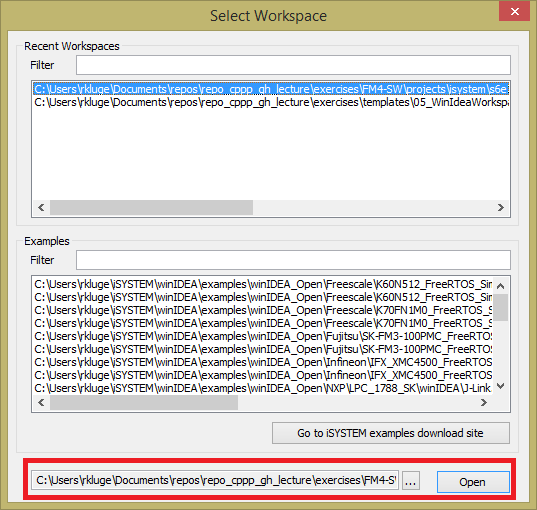
\includegraphics[width=.5\textwidth]{./05_c/figures/WinIDEASelectWorkspace.png}
\caption{Workspace-Auswahl in WinIDEA}
\label{fig:WinIdeaSelectWorkspace}
\end{centering}
\end{figure}

\item 
\RKi{Continue here: Überblick über IDE, Beispieprogramm öffnen, compilieren, downloaded, testen}
\end{enumerate}

\section{\ExercisePrefixEmbeddedC Taster abfragen \optional}

In dieser Aufgabe erweitern wir die vorherige Aufgabe um eine Benutzerinteraktion über den \textbf{User Button}.
Ziel dieser Aufgabe ist es, mit dem User Button die RGB-LED in zwei verschiedenen Szenarien zu kontrollieren.
Bei ersten Szenario soll es möglich sein die LED per Lichtschalter an und auszuschalten und beim zweiten Szenario soll die LED immer dann leuchten, wenn der \textbf{User Button} gedrückt ist.

\begin{enumerate}
\item 
Zunächst werden wir die nötigen Variablen in \textbf{button.h} deklarieren. Lege dir in der bekannten Weise zwei Zeiger auf die Direction und Value Register der blauen LED an. Weiterhin soll für den Lichtschalter der aktuelle Zustand der LED in einem unsigned 8 Bit Integer \textbf{LEDstatus} gespeichert werden.

\item Als User Button soll der digitale Button des Joystick 1, welcher an den Pin F5 des Mikrocontrollers angeschlossen ist, verwendet werden. Die Funktion \textbf{initLED()} soll den LED-Status, den Pin F5 und die blaue LED initialisieren. Der LED-Status soll zu Beginn 0 sein, und Pin F5 soll durch die Methode \textbf{Gpio1pin\_InitIn(pin, option) }initialiseren werden. Diese Funktion ist eine weitere Möglichkeit Pins des Mikrocontroller zu initialiseren. \textbf{Gpio1pin\_InitIn} intialisiert einen Pin als Eingang und kann zusätzlich zu diesem einen Pull-Up-Widerstand schalten, um das ankommende Signal zu verstärken. Der Name des Pins kann mit \textbf{GPIO1PIN\_PF5} angegeben werden und Pull-Up kann mit \textbf{Gpio1pin\_InitPullup(1u)} aktiviert werden. Abschließend soll die blaue LED in der dir bekannten Weise initialisiert werden. 

\item Mit \textbf{toggleBlueLED()} soll es möglich sein den Status der LED zu verändern. Demnach soll bei jedem Aufruf von \textbf{toggleBlueLED} der aktuelle Wert des Status invertiert werden. Der aktuelle Status der LED kann mit \textbf{setBlueLED(uint8\_t status)} gesetzt werden. 

\item Mithilfe der zuvor implementierten Funktionen sollen nun \textbf{ButtonToggleBlueLED()} und \textbf{ButtonHoldBlueLEDOn()} implementiert werden. \textbf{ButtonToggleBlueLED()} soll dem Button die Funktion eines Lichtschalters geben und  \textbf{ButtonHoldBlueLEDOn()} soll die LED zum leuchten bringen, solange der Button gedrückt gehalten wird. 

\end{enumerate}
\hints{
	\item Mit dem Aufruf \textbf{Gpio1pin\_Get(GPIO1PIN\_PF5)} kann der aktuelle Wert des Pin F5 ausgelesen werden.
	
	\item Es ist zu beachten, dass durch einen Pull-Up-Widerstand, sich die Spannung am Mikrocontroller invertiert. Folglich ist bei gedrückten Joystick das Eingangssignal am Mikrocontroller 0 und bei losgelassenem Button 1. 
	
	\item \textbf{while(Gpio1pin\_Get(GPIO1PIN\_PF5) == 0)} kann verwendet werden, um das Programm solange zu pausieren bis der Button losgelassen wird. 
}

\section{\ExercisePrefixEmbeddedC Touchdisplay ansteuern \optional}

\RKi{Ziel: (i) Regelmäßiges Muster ausgeben (Schachbrett, Blockschachbrett,...); (ii) Text ausgeben (s. writeText(char[]))}

\section{\ExercisePrefixEmbeddedC Joysticks abfragen \optional}

\RKi{Ziel: (i) Joystick-Daten auslesen und (ii) auf dem Display ausgeben. Die Studenten können entweder ihr eigene writeText-Funktion nutzen oder auf die Musterlösung der vorirgen Aufgabe zugreifen.}
\section{\ExercisePrefixEmbeddedC Touchscreen ansteuern \optional}
Eingebaut im mit dem Mikrocontroller verbundenen Bildschirm ist eine resistive 4-Wire Touchschicht.
Der Name setzt sich zusammen aus den Eigenschaften dieser Schaltung.
Resistiv steht für die Messung von Widerständen zum Erkennen von Touch-Gesten und 4-Wire, da für diese Durchführung vier Datenleitungen gebraucht werden.
Ein resistiver 4-Wire-Touchscreen ist wie in \Cref{fig:rsTouch} aufgebaut.
%
\begin{figure}[htbp]
    \centering
    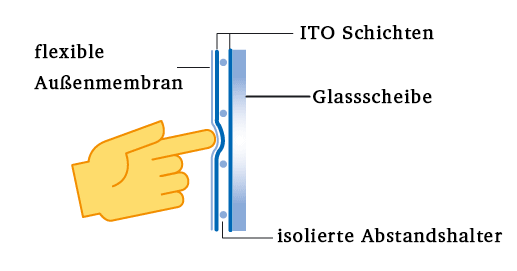
\includegraphics[width=0.35\textwidth]{./05_c/figures/4WireRSTouch.png}
    \caption{Aufbau eines resistiven Touchscreens}
    \label{fig:rsTouch}
\end{figure}
%
Dieser besteht aus
\begin{inparaenum}
\item
einer Glas- oder Acryl-Schicht,
\item 
einer äußeren resistiven Schicht die mit Indium-Zinn-Oxid (\enquote{indium tin oxide}, ITO) beschichtet ist,
\item 
isolierenden Punkten,
\item 
der inneren resistiven Schicht aus ITO und 
\item
einem Polyester-Film.
\end{inparaenum}
Die beiden resistiven Schichten sind jeweils an 2 Polen angeschlossen (\Cref{fig:fourRSTouch}).
%
\begin{figure}[htbp]
    \centering
    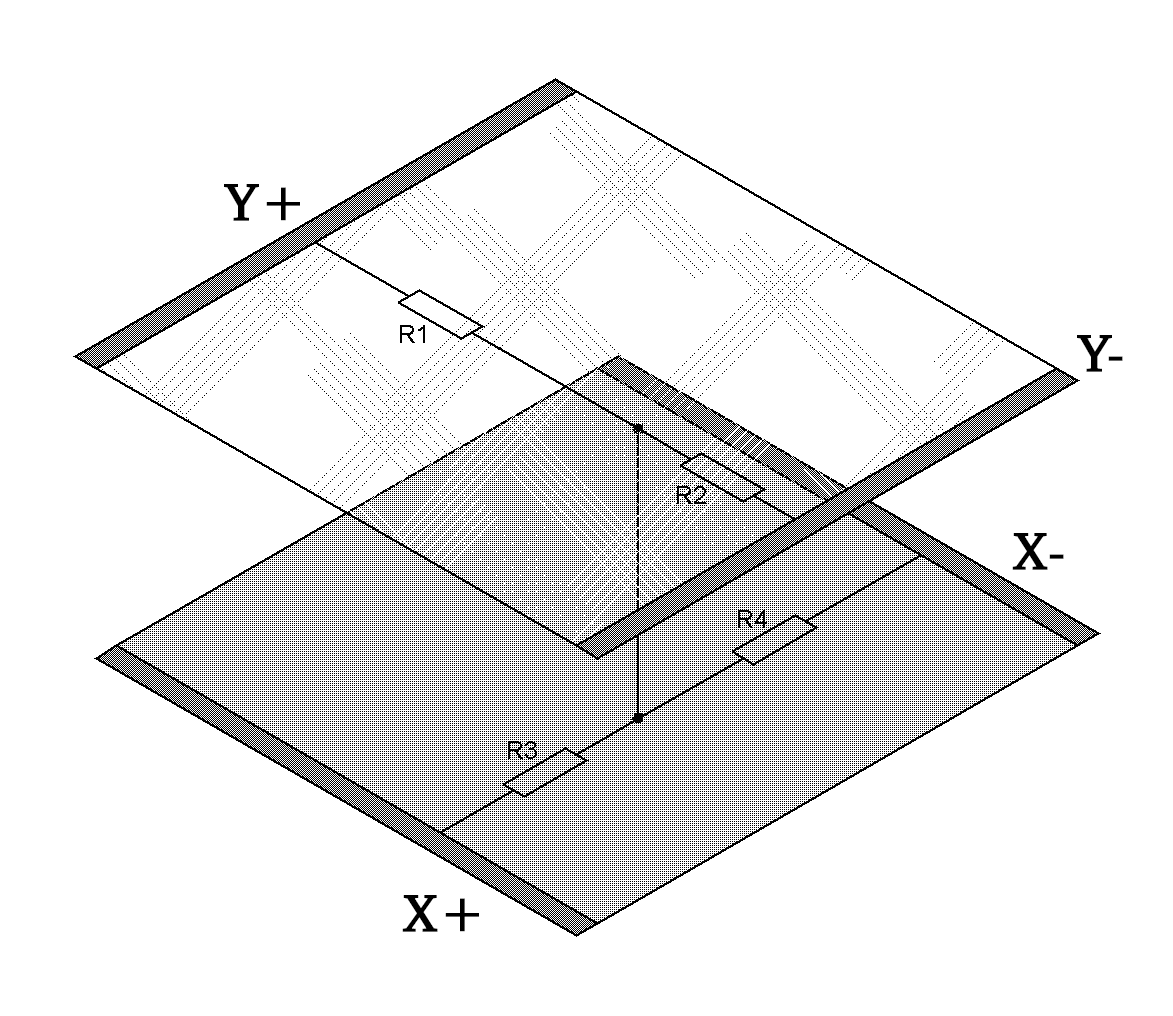
\includegraphics[width=0.3\textwidth]{./05_c/figures/ResistiveTS.png}
    \caption{Aufbau eines 4-Wire resistiven Touchscreens }
    \label{fig:fourRSTouch}
\end{figure} 
%
Die Schichten sind in Bezug auf ihre Pole um 90 Grad zueinander gedreht.
Dies ist wichtig, um später die X- und Y-Koordinaten des Druckpunkts zu lesen.
Sobald ein Objekt die oberste Glas- oder Acryl-Schicht berührt und genügend Druck ausübt, wird sich die oberste ITO-Schicht mit der unteren verbinden.
Die X- und Y-Koordinate des Druckpunkts wird bestimmt, indem die Spannungen an den Polen gemessen werden.
Zur Messung des X-Wertes werden X+ und X- über Gleichspannung geschaltet.
Das heißt, X+ ist beispielsweise auf Vcc und X- ist mit GND verbunden.
Durch die Verbindung der beiden ITO-Schichten entsteht ein Stromfluss durch beide Schichten und es kommt zu einem Spannungsteiler in der X-Schicht.
Die Spannungen zwischen X+ und dem Druckpunkt sowie dem Druckpunkt und X- lassen sich durch das Ausmessen von Y- und Y+ auslesen.
Diese Information wird vom Microcontroller ausgelesen, der die gemessene Spannung in Relation zur Auflösung des Displays setzt.
Die Y-Koordinate wird gemessen, indem Y+ und Y- an eine Gleichspannung gelegt und die Spannungen an X+ und X- ausgelesen werden.

Für dein Projekt stellen wir dir die Funktionen \lstinline|readTouchX()|, \lstinline|readTouchY()| und \lstinline|readTouchZ()| zur Verfügung, die X-, Y- und Z-Werte eines Druckpunkts auf dem Touchscreen auslesen können (\filename{analog.h}).
Ist der Z-Wert größer als ein bestimmter Grenzwert, kann von einer Berührung des Touchscreens ausgegangen werden. 


\subsection{Werte des Touchscreens debuggen}
Implementiere zunächst die Funktion \lstinline|debugTouch()|, die kontinuierlich die X-,Y- und Z-Werte des Touchscreens auf dem Bildschirm ausgibt.

\subsection{Zeichnen auf dem Touchscreen}
In diesem Abschnitt implementierst du eine kleine Mal-Anwendung für den Touchscreen.
Mit dieser soll es möglich sein, verschiedene Farben auszuwählen und mithilfe des Fingers auf dem Bildschirm zu zeichnen.
Vervollständige hierfür die Funktion \lstinline|paintTouch()|.
Bereits implementiert sind die Farbpaletten und der Lösch-Button auf der unteren Seite des Bildschirms.
Die Funktion \lstinline|printTouch()| muss noch um eine Touch-Logik ergänzt werden, die Berührungspunkte auf dem Bildschirm erkennt und diese korrekt interpretiert.
Hierbei gibt es folgende Szenarien:
\begin{itemize}
\item 
Die Farbpalette wird berührt und somit verändert sich die aktuelle Malfarbe.
\item 
Bild erneuern wurde gedrückt und der Malbereich wird zurückgesetzt.
\item 
Wird der freie Zeichen-Bereich berührt, so soll an dieser Stelle in der ausgewählten Farbe ein ausgefüllter Kreis mit dem Radius \lstinline|PENRADIUS| gezeichnet werden.
\end{itemize}
\Cref{fig:paintTouch} zeigt, wie die Anwendung fertig aussehen kann.
\begin{figure}[htbp]
	\centering
	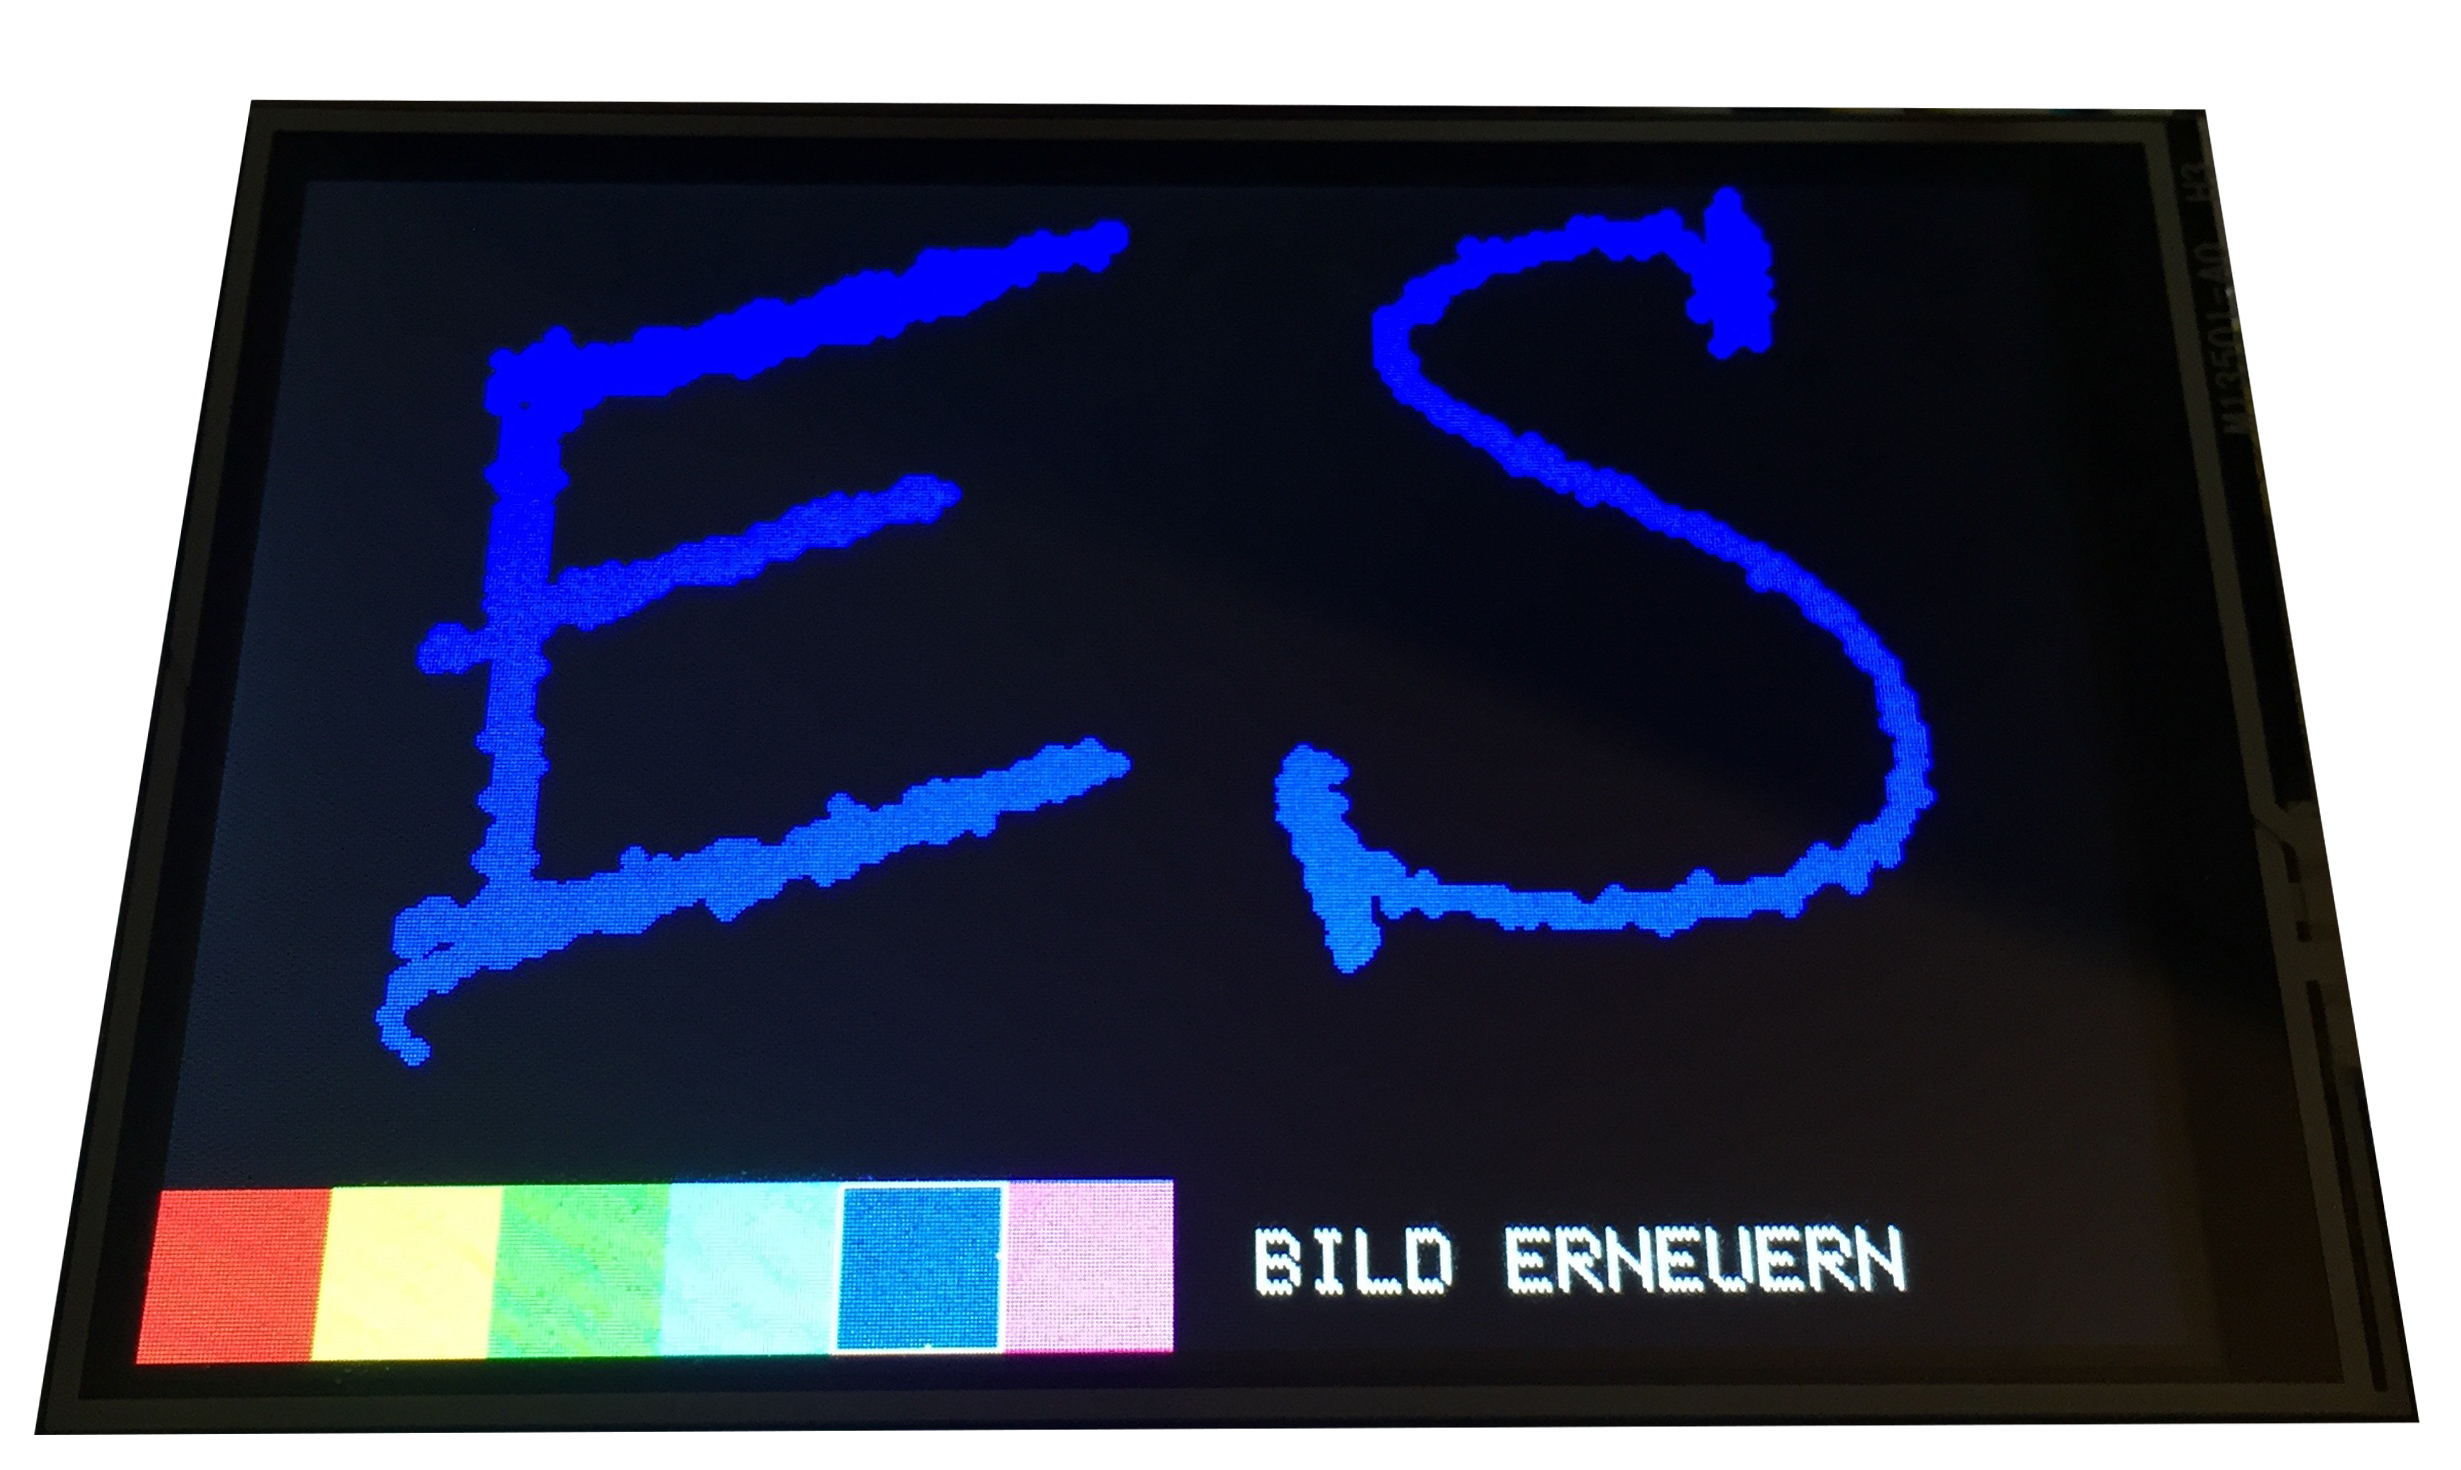
\includegraphics[width=0.3\textwidth]{./05_c/figures/Paint-Szenario.png}
	\caption{Mal-Anwendung auf dem Touchscreen}
	\label{fig:paintTouch}
\end{figure} 
\section{\ExercisePrefixEmbeddedC Eigenes Microcontroller-Projekt umsetzen \optional}

Nachdem du einige der Ein- und Ausgabemöglichkeiten des Boards kennengelernt hast, besteht deine Aufgabe in diesem Teil darin, ein kleines Projekt deiner Wahl umzusetzen.
Du hast hierbei die freie Wahl, die folgenden Vorschläge sollen nur als Anregung dienen.

\subsection*{Vorschlag: Pong}
Zwei Gegner sollen je einen Balken (Rechteck) am linken oder rechten Rand des Spielfeldes mit den Schiebereglern steuern können, um einen Ball (ein Quadrat) im Spiel zu halten.
Erreicht der Ball den linken oder rechten Rand des Spielfelds, so bekommt der Spieler auf der anderen Seite einen Punkt und der Ball wird an seine Anfangsposition (die Mitte des Spielfelds) zurückversetzt.
Erreicht der Ball den oberen oder unteren Rand sowie einen der Balken der Spieler, so wird der Ball reflektiert - verlässt also niemals das Spielfeld.

Gewonnen hat der Spieler, der zuerst eine definierte Anzahl an Punkten erreicht.
Die aktuelle Punktzahl beider Spieler könnte auf der Siebensegmentanzeige ausgegeben werden.
\begin{center}
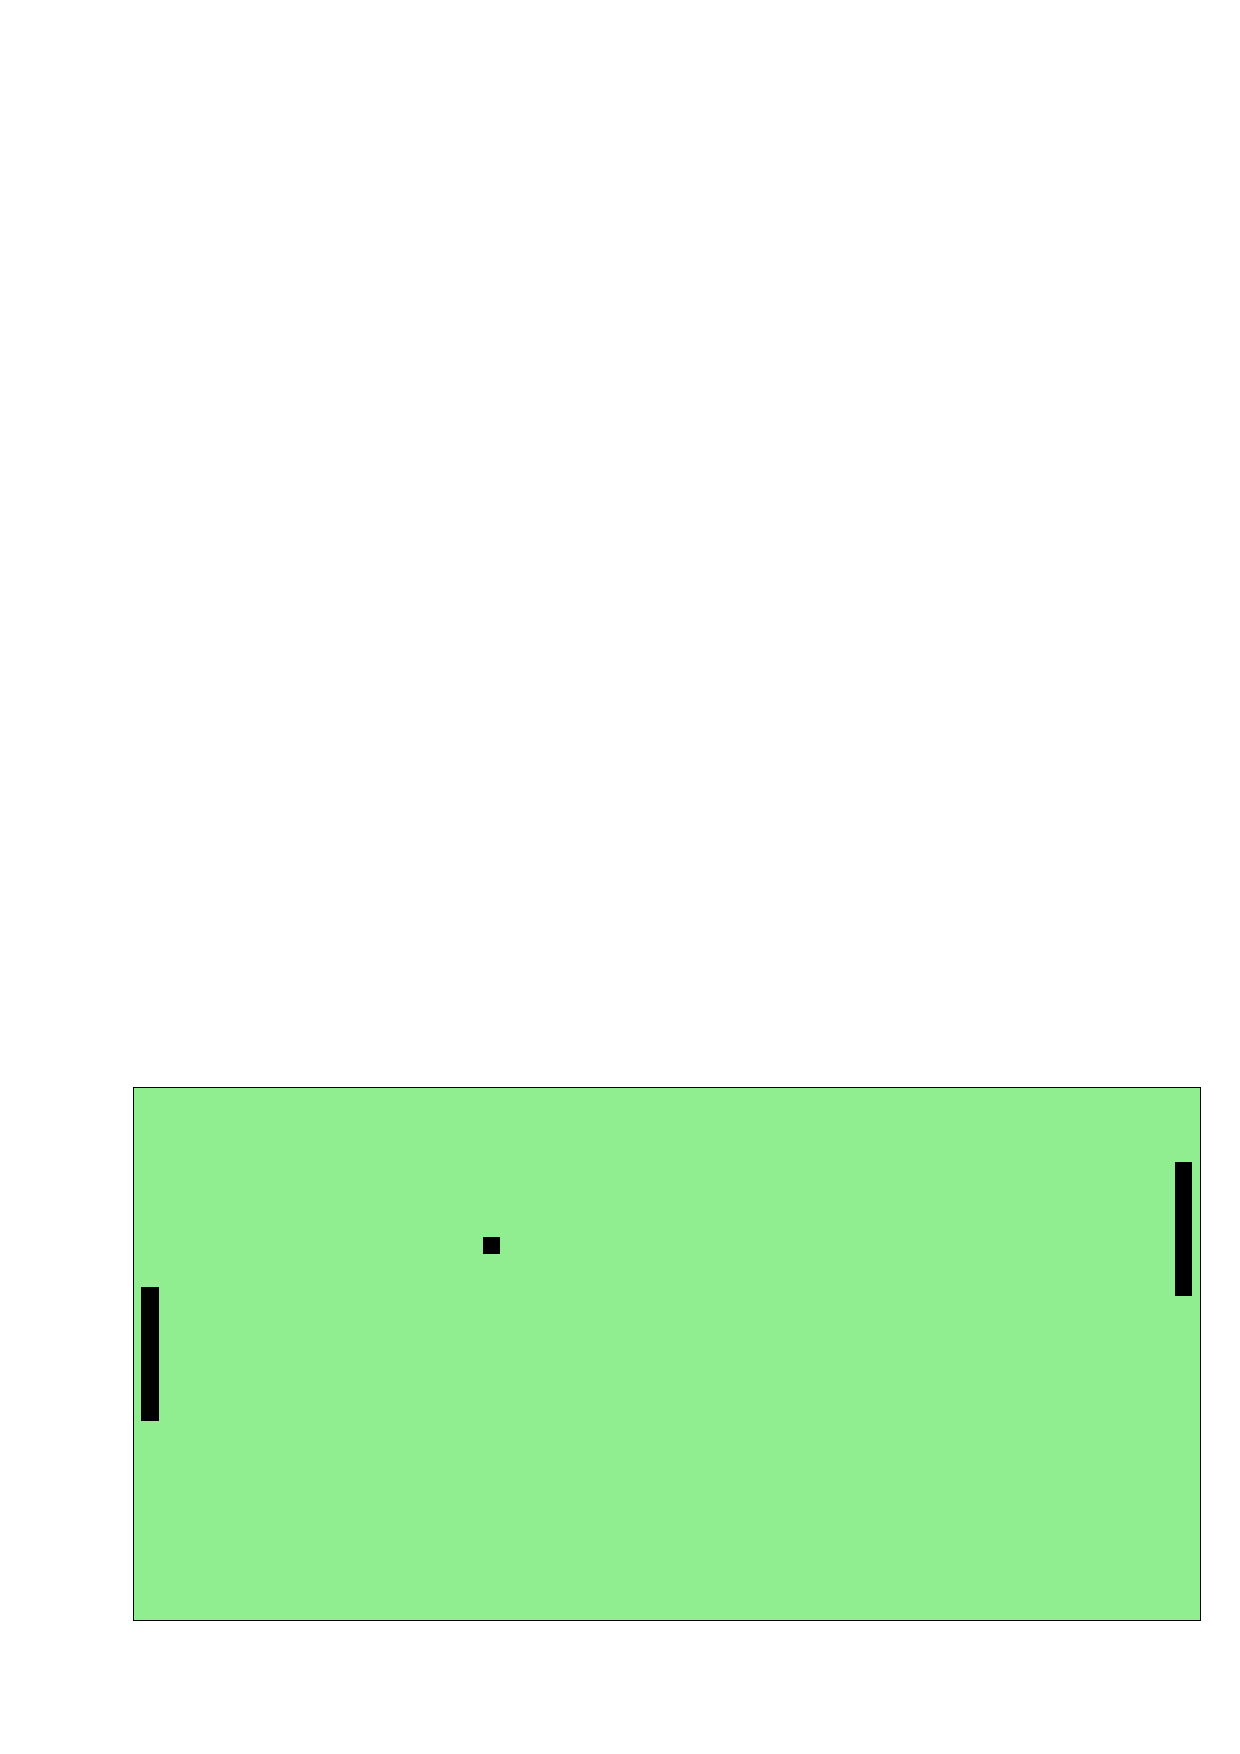
\includegraphics[scale=0.4]{05_c/figures/pong}
\end{center}



\subsection*{Vorschlag: Game of Life}
\glqq{}Game of Life\grqq{}\footnote{siehe auch \url{http://de.wikipedia.org/wiki/Conways_Spiel_des_Lebens}} besteht aus einem zweidimensionalen Spielfeld.
Jedes Feld steht für eine Zelle, die \textit{tot} (grün) oder \textit{lebendig} (schwarz) ist.
Jede Zelle hat acht Nachbarzellen, die ebenso tot oder lebendig sein können.
Zu Beginn gibt es eine vordefinierte Anfangsgeneration.
%
Durch festgelegte Regeln wird die nachfolgende Generation ermittelt:
\begin{itemize}
	\item Eine \textbf{lebende Zelle} \dots
	\begin{itemize}
		\item mit 1 oder 0 lebenden Nachbarn stirbt aus Einsamkeit.
		\item mit 4 oder mehr lebenden Nachbarn stirbt wegen Übervölkerung.
		\item mit 2 oder 3 lebenden Nachbarn bleibt am Leben.
	\end{itemize}
	\item Eine \textbf{tote Zelle} mit genau 3 lebenden Nachbarn wird in der nächsten Generation geboren werden, andernfalls bleibt sie tot.
\end{itemize}
%
Als Anfangsgeneration eignen sich zufällige Populationen oder eine der folgenden Figuren:
\begin{center}
	
\includegraphics[scale=1]{05_c/figures/gol_init1}
	\hspace{5mm}
	
\includegraphics[scale=1]{05_c/figures/gol_init2}
	\hspace{5mm}
	
\includegraphics[scale=1]{05_c/figures/gol_init3}
\end{center}
%
\hints{
	\item Da das Spielfeld begrenzt ist, soll es torusförmig aufgebaut werden.
    Das heißt: Alles, was am unteren Rand des Spielfelds verschwindet, kommt oben wieder heraus -- das Gleiche gilt für den linken und rechten Rand. 
	\item Verwende als Spielfeld ein mehrdimensionales Array
	\item Ein weiteres mehrdimensionales Array bietet sich an, um die zukünftige Generation erzeugen zu können.
	\item Achte beim torusförmigen Feld unbedingt darauf, dass du nicht über die Grenzen des Spielfelds hinaus zugreifst!
    Das kann zu unvorhersehbarem und schwer zu debuggenen Verhalten des ganzen Displays führen!
}

\subsection*{Vorschlag: Regentropfen}

Das Touch-Display ist ein kleiner Teich;
wenn du eine Stelle mit dem Finger berührst, breitet sich von dort eine konzentrische Welle aus.
Die Geschwindigkeit der Welle kannst du zusätzlich abhängig machen vom ausgeübten Druck.


\subsection*{Weitere Vorschläge}
\RKi{Beispielbilder finden, CC4.0-kompatibel sind}
\begin{minipage}{.45\textwidth}
    \begin{center}Asteroids\\\vspace{4ex}
        %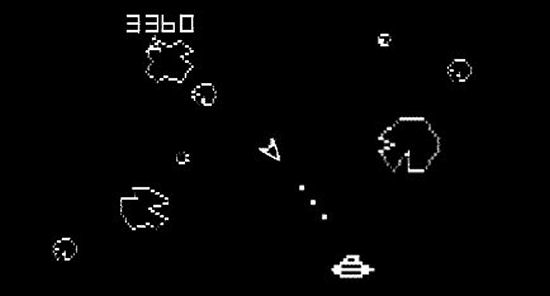
\includegraphics[width=.5\textwidth]{05_c/figures/img_asteroids.png}
    \end{center}
    \begin{center}Pacman\\\vspace{4ex}
        %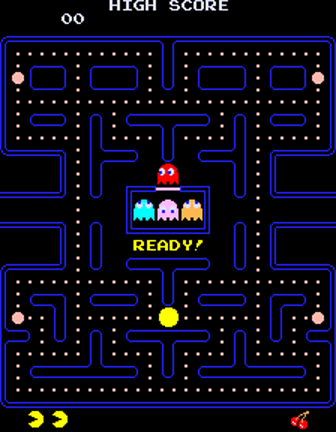
\includegraphics[width=.3\textwidth]{05_c/figures/img_pacman.png}
    \end{center}
    \begin{center}Labyrinth\\\vspace{4ex}
        %
\includegraphics[width=.4\textwidth]{05_c/figures/img_maze.png}%
    \end{center}
\end{minipage}
\begin{minipage}{.45\textwidth}
	\begin{center}Ausweichspiele à la Hugo\\\vspace{4ex}
        %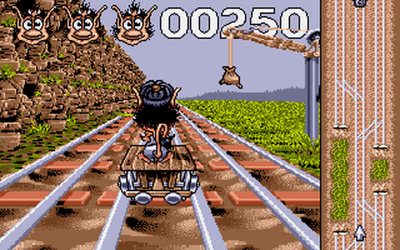
\includegraphics[width=.4\textwidth]{05_c/figures/img_hugo.png}
    \end{center}
	\begin{center}Moorhuhn\\\vspace{4ex}
        %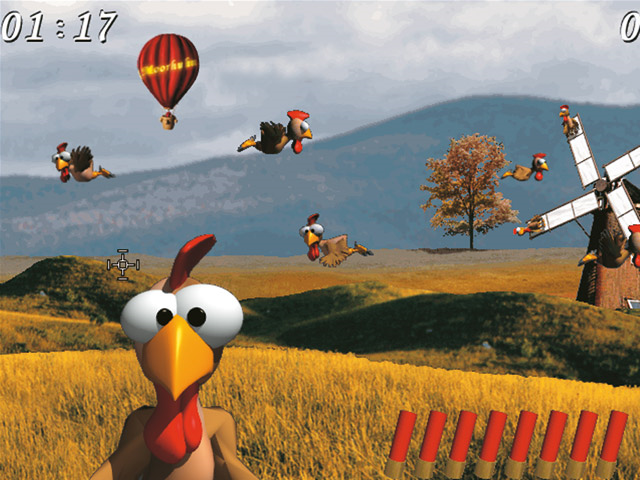
\includegraphics[width=.4\textwidth]{05_c/figures/img_moorhuhn.png}
    \end{center}
	\begin{center}Snake\\\vspace{4ex}%
       % 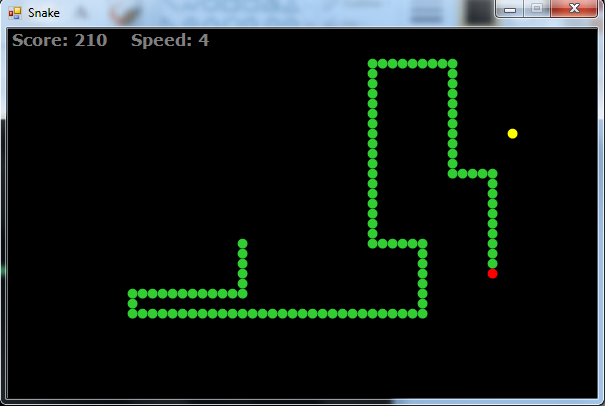
\includegraphics[width=.4\textwidth]{05_c/figures/img_snake.png}
    \end{center}
\end{minipage}


\hints{
	\item Möchte man ein Bild auf dem Board anzeigen, so empfiehlt es sich die einzelnen Pixeldaten in einem Array zu speichern.
	GIMP bietet hierfür die Möglichkeit eine Bilddatei als Header im \texttt{GIMP header image file format} zu exportieren.
	Da das Board nur zwei Farbwerte ermöglicht, sollte das Bild vor dem Exportieren über den Menüpunkt \textbf{Bild --> Modus} auf \textbf{indiziert \ldots} (Schwarz/Weiß-Palette (1-Bit)) gestellt werden.
	Anschließend kann man das \lstinline{header_data} Array verwenden, um auf die Bilddaten zuzugreifen.
}

% !TeX spellcheck = de_DE
\section{\ExercisePrefixEmbeddedC DHT11 \optional}

\optionaltextbox

Für die folgende Aufgabe musst du dir folgendes zusätzliches Material bei den Betreuern beschaffen:
\begin{itemize}
\item DHT11 Temperatur- und Feuchtigkeitssensor
\item 3 Steckbrücken Pin-Pin 20cm (jeweils ein verbundenes Steckbrückenpaar und eine einzelne Steckbrücke)
\item 1 Steckbrücke Pin-Buchse 20cm
\item 1 Widerstand \SI{10}{\kilo\ohm} (oder höher)
\end{itemize}

Der DHT11 ist ein Temperatur- und Feuchtigkeitssensor, der mithilfe des Steckplatine an den Microcontroller angeschlossen werden kann.
Der DHT11 hat 4 Anschlüsse (Pins), von denen im Rahmen des Praktikums 3 verwendet werden.
Zwei Pins werden für Masse (\lstinline|GND|) und Versorgungsspannung (\lstinline|VCC|) genutzt und ein Pin für die digitale Datenübertragung zwischen dem DHT11 und dem Microcontroller.
Abbildung \ref{fig:dht11Pins} zeigt die Pin-Belegung des DHT11.
Pin 1 wird mit \lstinline|VCC| verbunden und Pin 4 mit \lstinline|GND|.
Pin 2 ist ein I/O-Pin zur digitalen Datenübertragung.
In dieser Aufgabe ist es das Ziel die Temperatur- und Feuchtigkeitswerte des Sensors kontinuierlich auszulesen und diese auf dem Display darzustellen.
\begin{figure}[!htb]
	\centering
	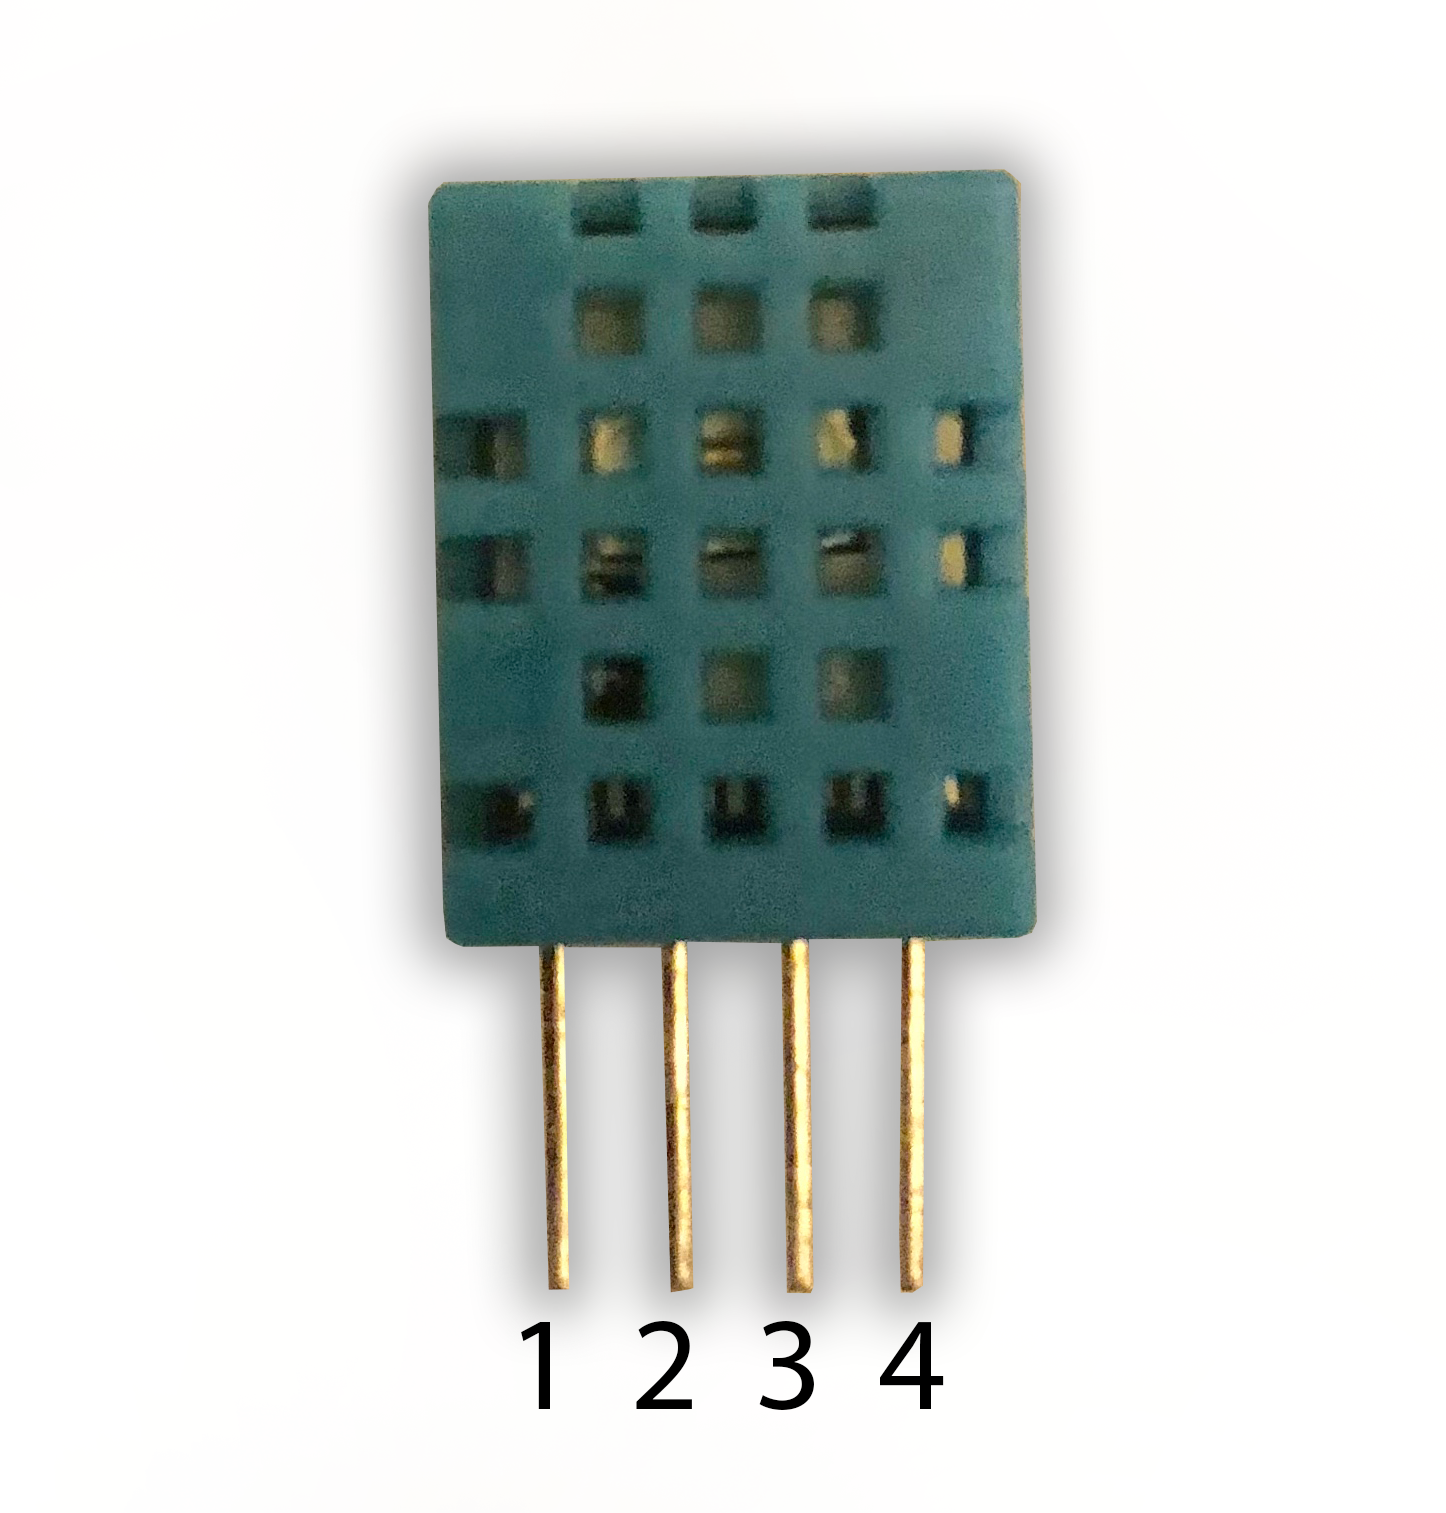
\includegraphics[width=0.2\textwidth]{./05_c/figures/DHT11.png}
	\caption{DHT11 Pinbelegung}
	\label{fig:dht11Pins}
\end{figure} 

\begin{enumerate}
\item 
Zunächst trenne den Microcontroller von der Stromzufuhr und stelle sicher, dass dieser ausgeschaltet ist.
Verbinde gemäß Abbildung \ref{fig:dht11Schematics} den DHT11 mit dem Microcontroller.
Der DHT11 wird, von links gezählt, an den dritten Pin des CN17 Steckers des Microcontrollers angeschlossen (Port 5, Pin 2, Präprozessorkonstante \lstinline|GPIO1PIN_PF52|).
Nutze als Unterstützung Abbildung~\ref{fig:cpppWiring}, die schematisch die GPIO-Verbindungen des Microcontrollers darstellt.
Bevor der Microcontroller wieder an den Computer angeschlossen wird, lasse die Verkabelung von einem Tutor überprüfen.
%
\begin{figure}[!htb]
	\centering
	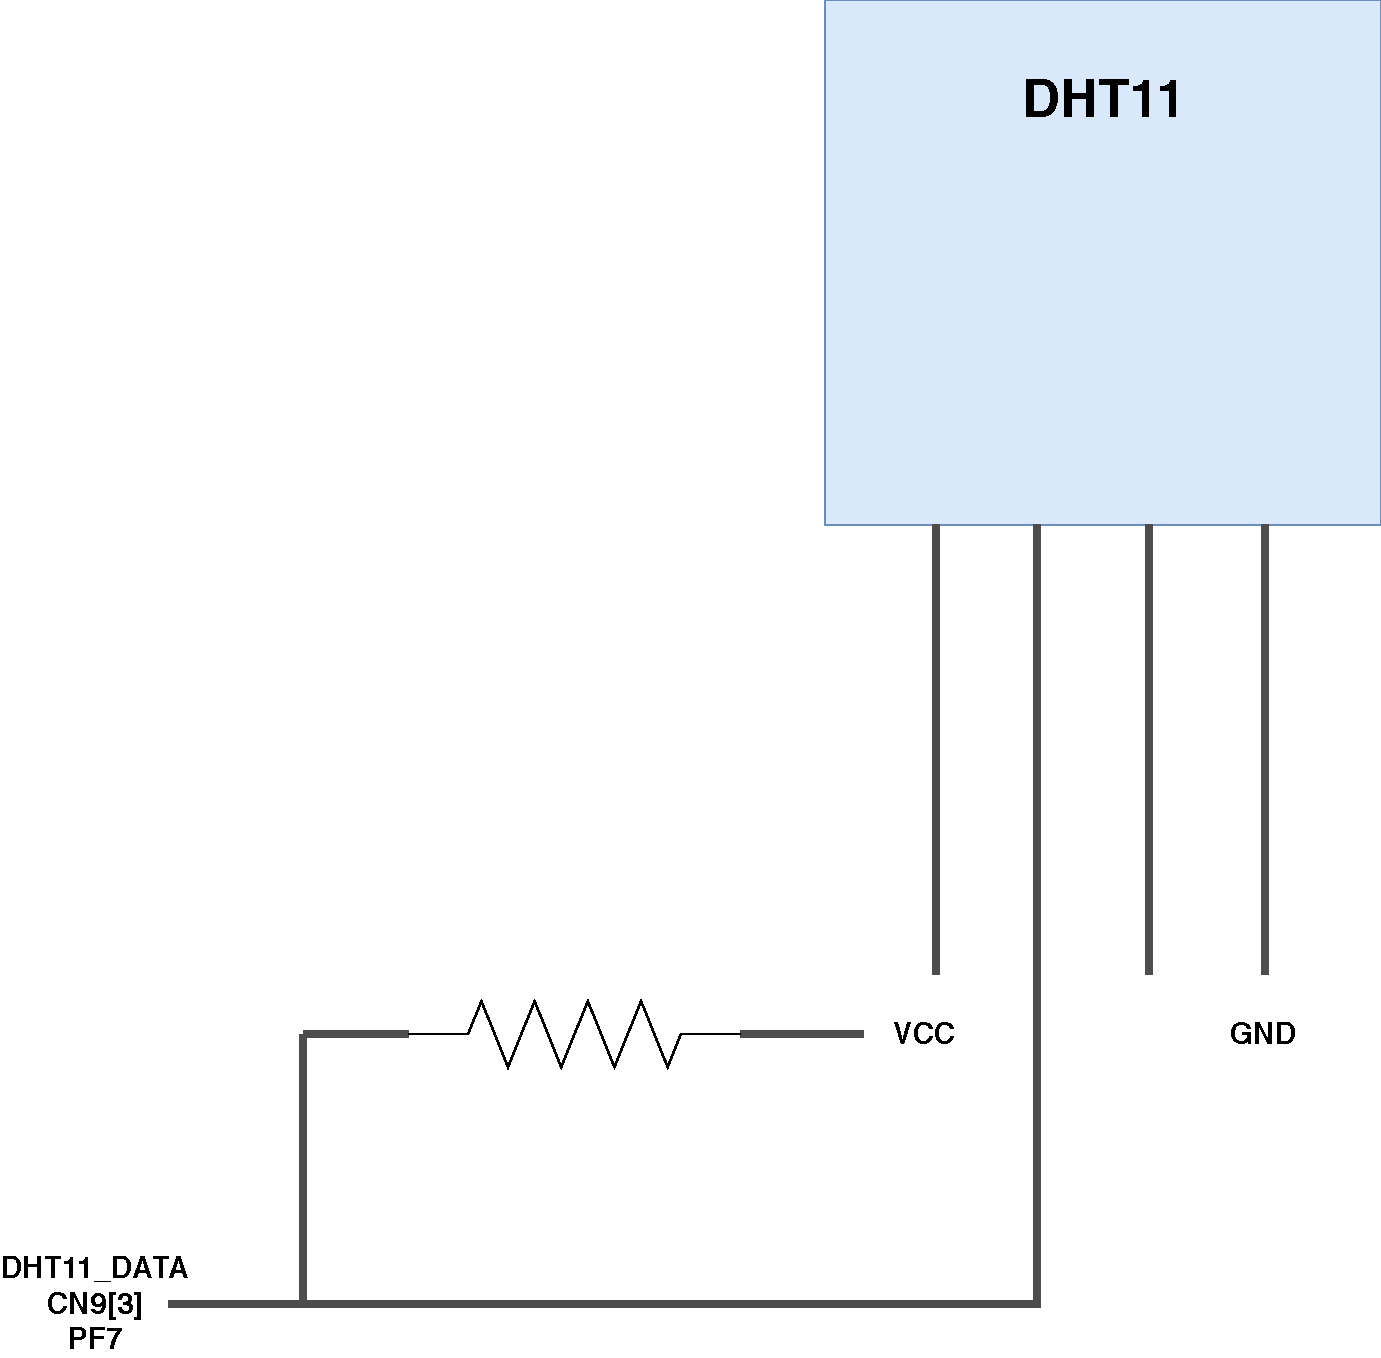
\includegraphics[width=0.35\textwidth]{./05_c/figures/DHT11-Schematics.pdf}
	\caption{Verkabelung des DHT11}
	\label{fig:dht11Schematics}
\end{figure} 
\begin{figure}[!htb]
	\centering
	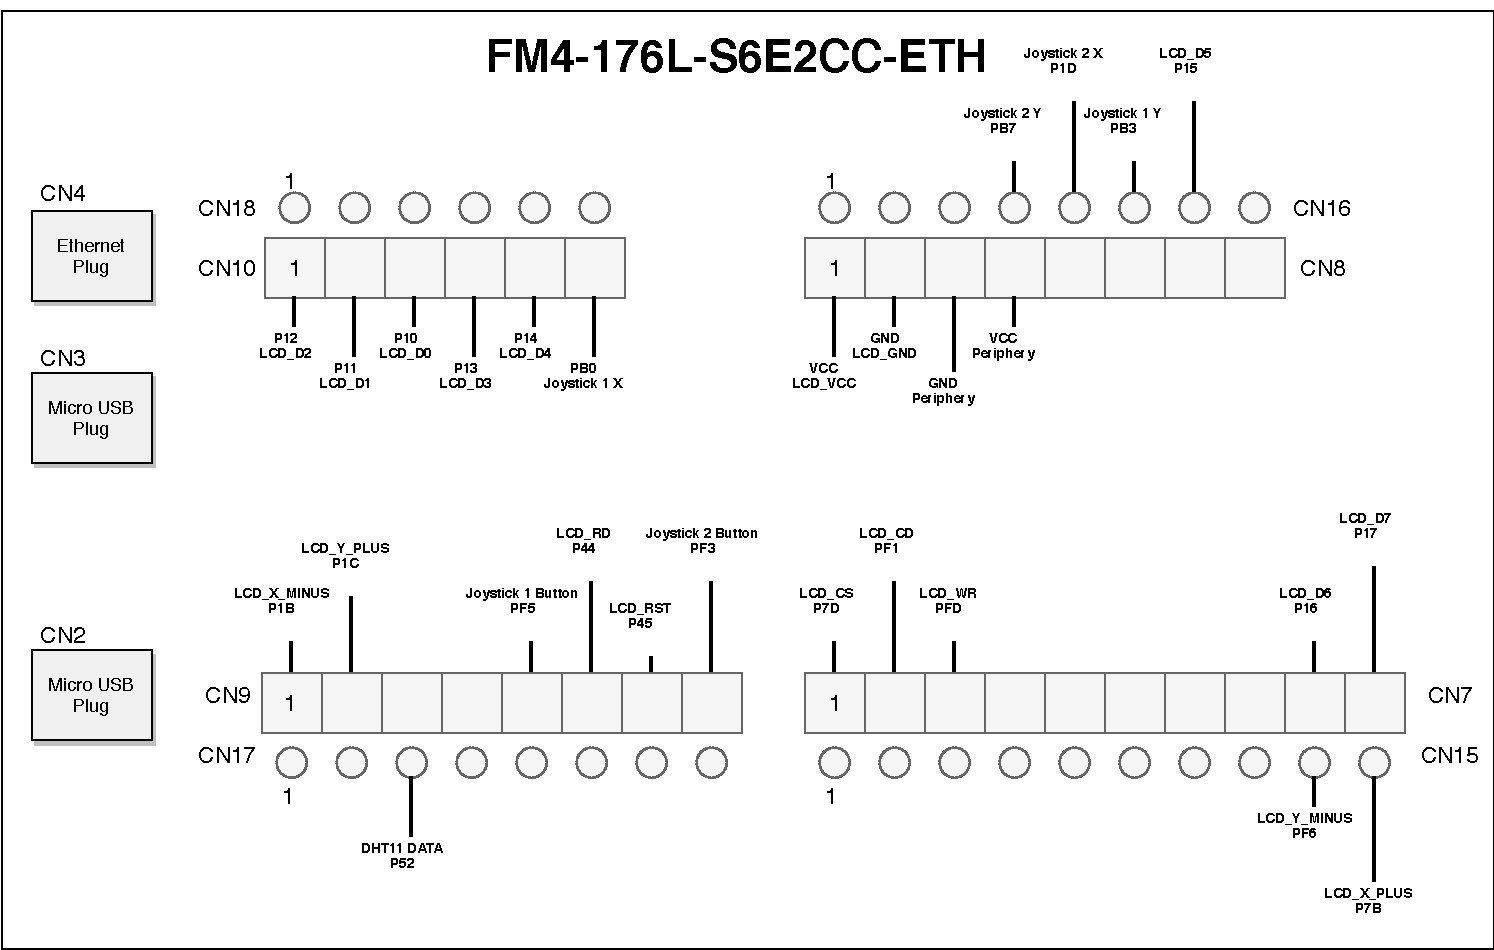
\includegraphics[width=0.7\textwidth]{./05_c/figures/cppp-wiring.pdf}
	\caption{Verkabelung des DHT11}
	\label{fig:cpppWiring}
\end{figure} 

\item 
In der Funktion \lstinline|readDHT11(uint8_t* humidity, uint8_t* temperature)| in der Datei \filename{dht11.c} wird zunächst eine Präambel vom DHT11 an den Microcontroller gesendet.
Hierdurch wird die Verbindung zwischen dem DHT11 und dem Microcontroller synchronisiert. 
Nach der Präambel beginnt der DHT11 40 Bits an den Microcontroller zu senden.
Abbildung \ref{fig:dht11Package} zeigt die Aufteilung der Bitgruppen.

Implementiere die fehlenden Stellen der Funktion \lstinline|readDHT11(uint8_t* humidity, uint8_t* temperature)|, indem du folgende Teilschritte umsetzt.
Nach der Präambel müssen zunächst die ankommenden Signale als 40~Bits interpretiert und in einem Array mit 5~Einträgen je 8~Bits gespeichert werden.
Lese mit \lstinline|Gpio1pin_Get(GPIO1PIN_P52)| den aktuellen Wert des digitalen Pins aus und entscheide entsprechend der folgenden Logik, ob es sich um eine 1 oder 0 handelt.
Ist der Pin länger als \SI{30}{\micro\second} auf \lstinline|HIGH| gesetzt $t_{HIGH} > \SI{30}{\micro\second}$, dann interpretiere dieses Signal als eine 1 und im umgekehrten Fall $t_{HIGH} < \SI{30}{\micro\second}$ als eine 0.
Nachdem alle 40 Bits empfangen wurden, bilde die Checksumme, welche die Summe der ersten 32 Bits darstellt. 
Ist der folgende Pseudocode erfüllt, dann ist die Übertragung der Daten erfolgreich gewesen.
%
\cpppInputListing{05_c/listings/dht11_checksum.c}
%
Beende die Methode  \lstinline|readDHT11readDHT11|, sofern die Checksumme nicht stimmt. 
Ist die Checksumme richtig, speichere die aktuelle Temperatur und Feuchtigkeit in den übergebenen Parametern \lstinline|humidity| und \lstinline|temperature|.
\begin{figure}[!htb]
	\centering
	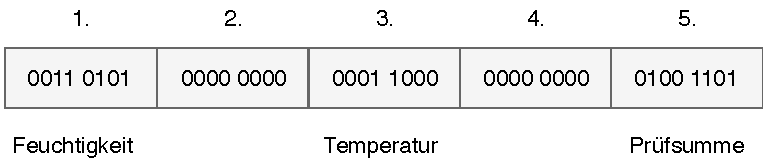
\includegraphics[width=0.7\textwidth]{./05_c/figures/dht11Bits.pdf}
	\caption{40 Bit Datenstruktur eines DHT11 Pakets}
	\label{fig:dht11Package}
\end{figure} 
\hints{
	\item Bei der Abfrage des Pins mithilfe von \lstinline|Gpio1pin_Get(GPIO1PIN_P52)|, kann es dazu kommen, dass fehlerhafte Signale dauerhaft auf \lstinline|HIGH| oder \lstinline|LOW| bleiben.
	Um diesen Fall zu filtern, verwende folgende Art der Abfrage.
	\cpppInputListing{05_c/listings/dht11.c}
	
	\item Um einen Delay auf dem Microcontroller ausführen, kannst du die Methode \lstinline|microDelay(uint32_t timeInMicroseconds)| verwenden. Zum Beispiel wird beim Aufruf  \lstinline|microDelay(20)| der Microcontroller \SI{20}{\micro\second} pausiert.
	
	\item Der DHT11 sendet immer seine Daten geordnet nach dem höchsten Bit, sodass der höchstwertigste Bit zuerst gesendet wird.
}

\item 
Nutze die Methoden \lstinline|writeTextln| und \lstinline|writeNumberOnDisplay| der Display-Library, um die Sensorenwerte auf dem Display auszugeben.

\hints{
	\item 
	Falls du die Funktionen \lstinline|writeTextln| und \lstinline|writeNumberOnDisplay| noch nicht implementiert hast, kannst du die Methoden der Musterlösung mit der Konkatenation des Suffix \lstinline|_s| nutzen (also bspw. \lstinline|writeTextln_s| und \lstinline|writeNumberOnDisplay_s|).
}

\end{enumerate}
\section{\ExercisePrefixEmbeddedC Beschleunigungssensor \optional}

% !TeX spellcheck = de_DE
\section{\ExercisePrefixEmbeddedC Android Bluetooth Low Energy \optional}
\newcommand{\toolAble}{\textsc{ABLE}\xspace}
\toolAble (Android Bluetooth Low Energy) ist eine Applikation für Androidgeräte, um über BLE (Bluetooth Low Energy) eine drahtlose Verbindung zwischen einem Android-Smartphone und einem anderen BLE-Gerät herzustellen.
Der Mikrocontroller des C/C++-Praktikums kann durch ein zusätzliches Modul mit BLE erweitert werden.
Du kannst auf einem Androidgerät die \toolAble-App installieren und dich mit dem Mikrocontroller verbinden.
\Cref{fig:ablePreview} zeigt ein Beispielprogramm, in dem der Mikrocontroller den X-Wert des Joysticks~1 über BLE an ein Android-Smartphone sendet.
Eine ausführliche Anleitung zur Nutzung von \toolAble auf dem Mikrocontroller des Praktikums findest du unter \href{https://github.com/Echtzeitsysteme/able/wiki/Cpp-Lab-Tutorial}{diesem Link [1]}. 
\begin{figure}[!htb]
	\centering
	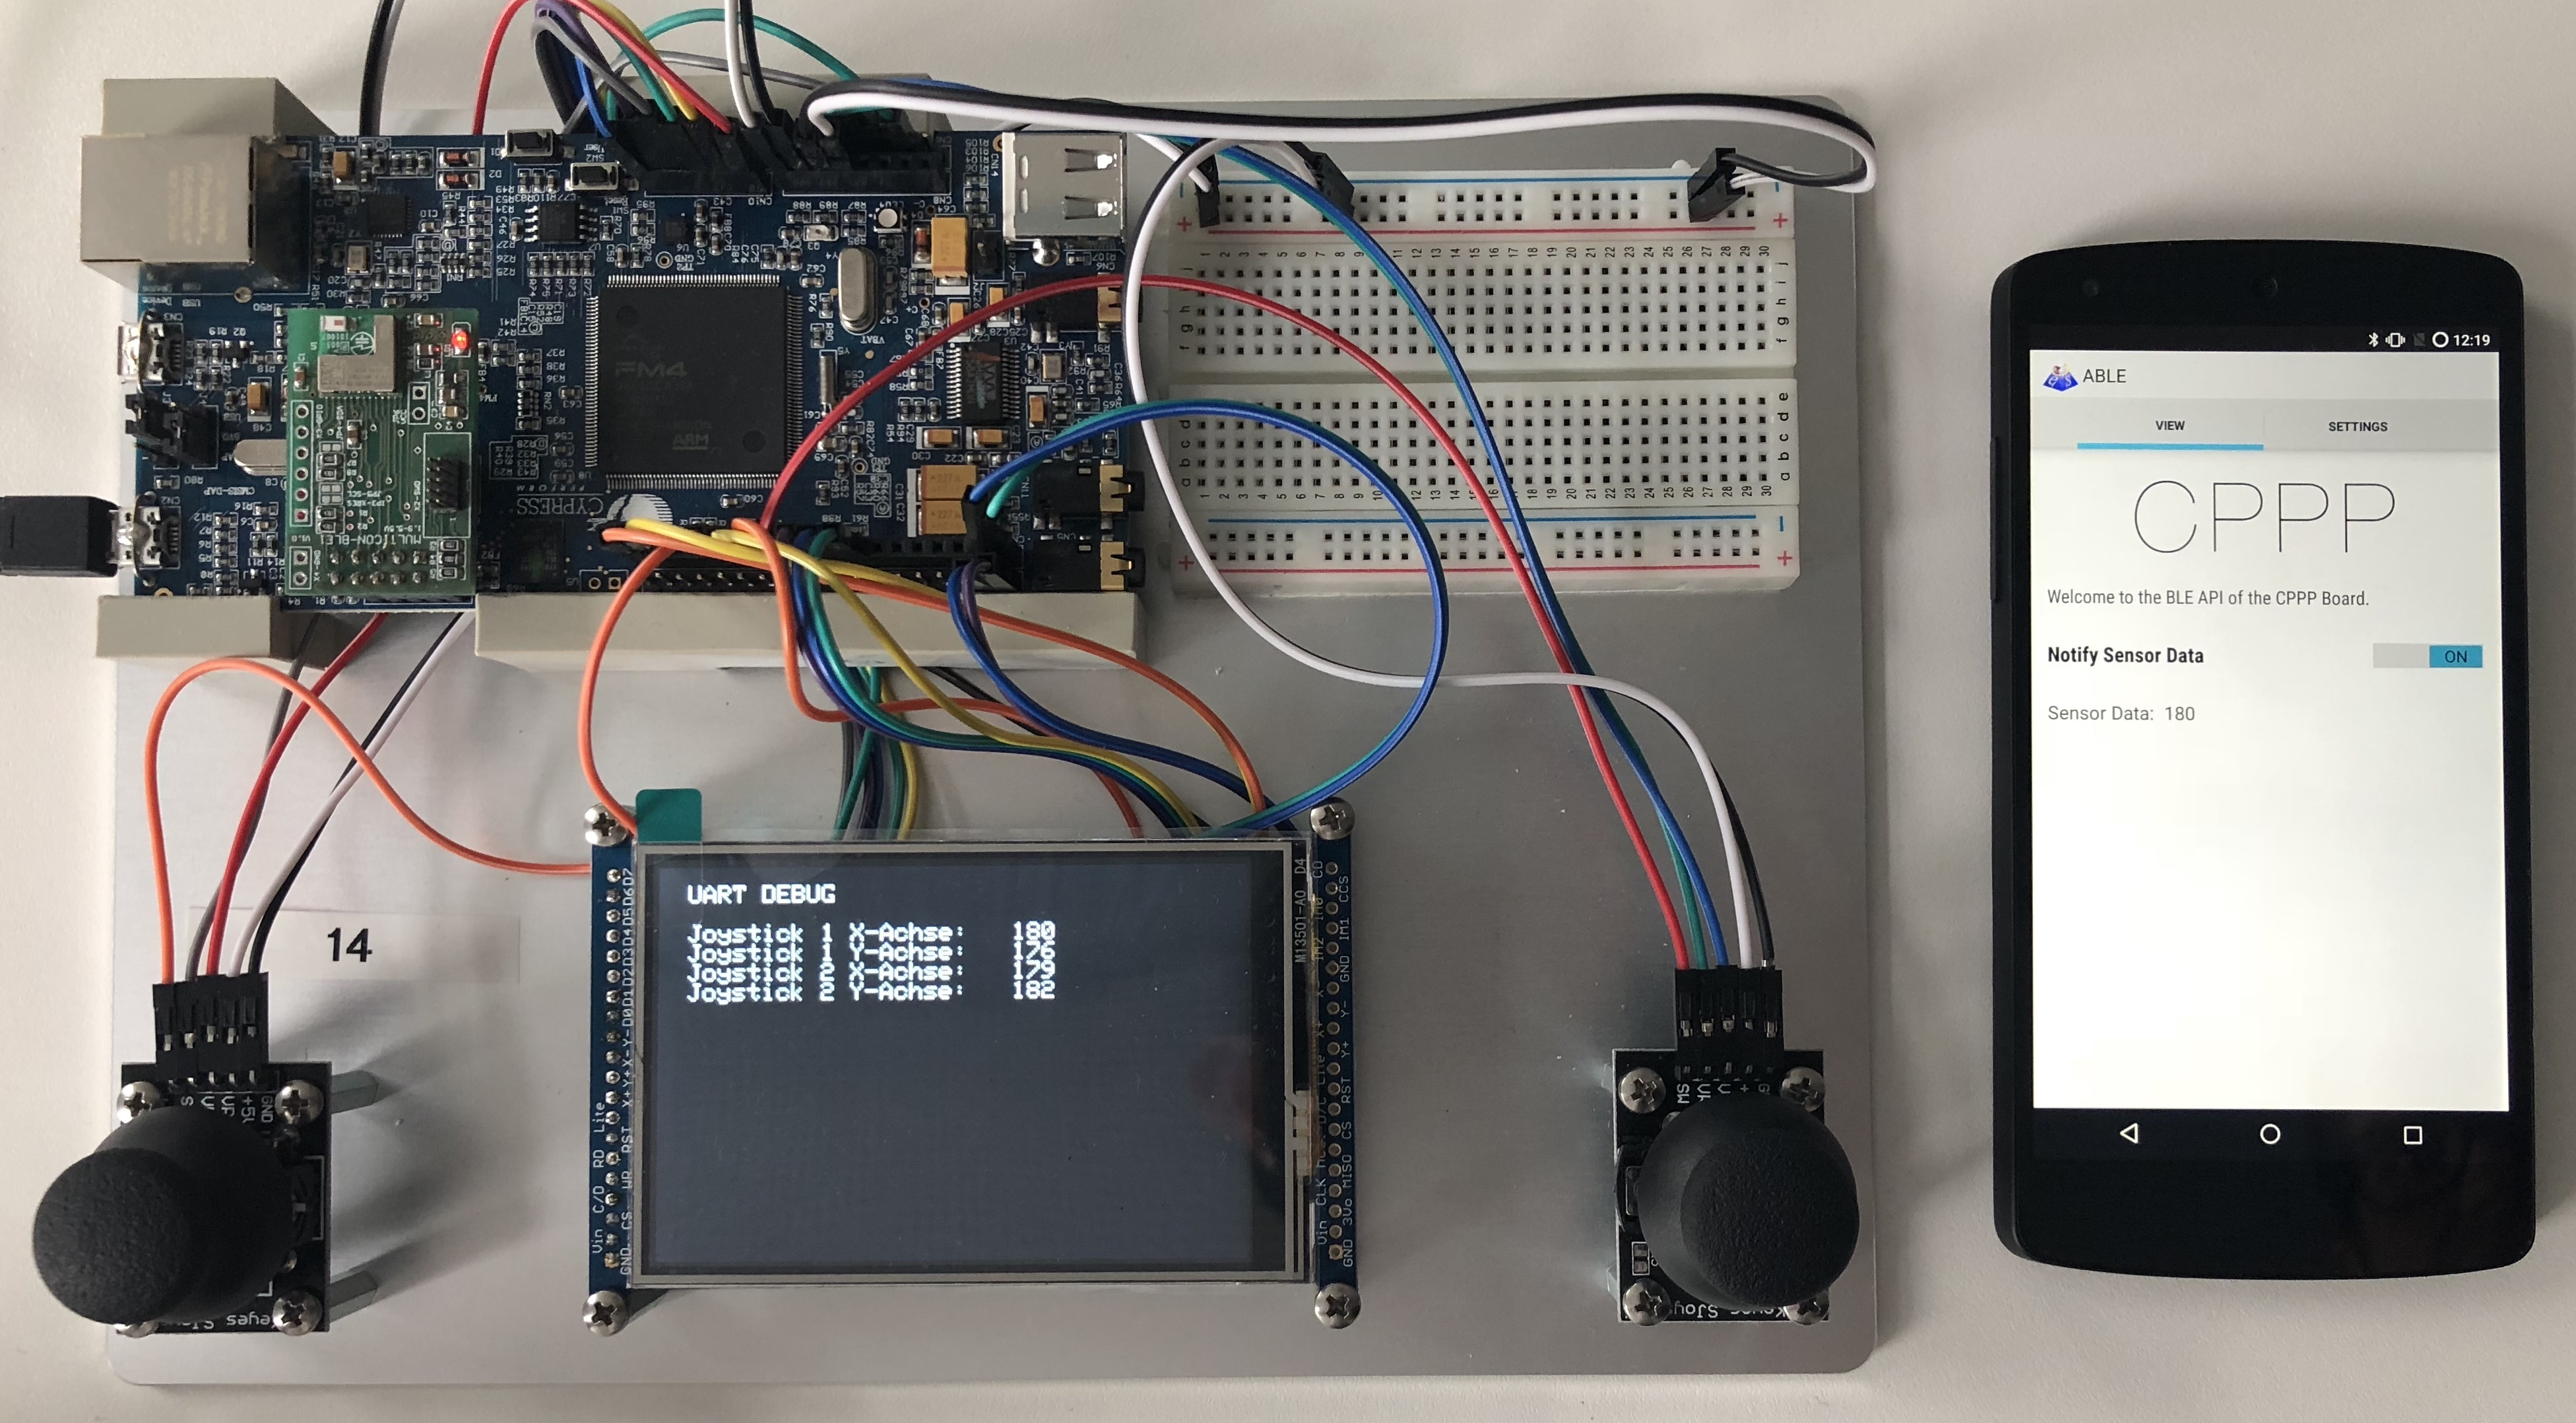
\includegraphics[width=0.9\textwidth]{./05_c/figures/ABLE_preview.jpg}
	\caption{\toolAble: Der Microcontroller verbunden über Bluetooth mit einem Androidgeräte}
	\label{fig:ablePreview}
\end{figure} 

% !TeX spellcheck = de_DE
\clearpage
\section{\ExercisePrefixEmbeddedC WSN---Wide Sensor Network\optional}
\newcommand{\toolWSN}{\textsc{WSN}\xspace}

Ein \toolWSN (Wide Sensor Network) ist ein Netzwerk aus verteilten Sensorknoten. Ziel dieser Aufgabe ist es, das Mikrocontrollerboard um weiteren Mikrocontroller mit WiFi-Schnittstelle zu erweitern, sodass mehrere Boards zusammen ein drahtloses Netzwerk (WLAN) aufspannen können, über welches gemessene Sensordaten an eine zentralen Server-Anwendung gesendet werden können.

Als Erweiterungsmodul nutzen wir das ESP-12E Modul. Dieses wird mit einer modifizierten Version der \href{https://github.com/martin-ger/esp_wifi_repeater}{esp\_wifi\_repeater-Firmware} zum Einsatz. Die Kommunikation zwischen unserem Mikrocontroller und dem ESP-Board wird über UART realisiert.

\begin{enumerate}
	\item Zuerst muss das ESP-Board wie in den beiden Abbildungen zu sehen angeschlossen werden. Dazu sind 4 Leitungen nötig: Masse (GND), Versorgungsspannung (Vcc) und je einmal von Tx (Transmit) zu Rx (Receive) und vice versa.
	
	\begin{minipage}{.5\textwidth}
		\centering
		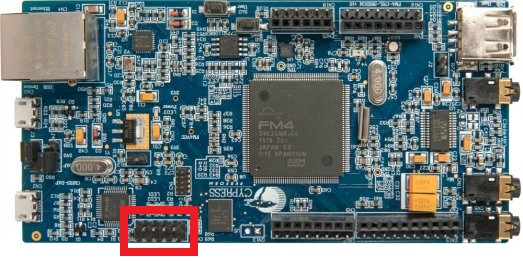
\includegraphics[width=\textwidth]{./05_c/figures/s6e2cc.jpg}
		%\captionof{figure}{Position des Pinheaders auf dem Board}
		%\label{fig:s6e2cc}
	\end{minipage}
	\begin{minipage}{.5\textwidth}		
		\centering
		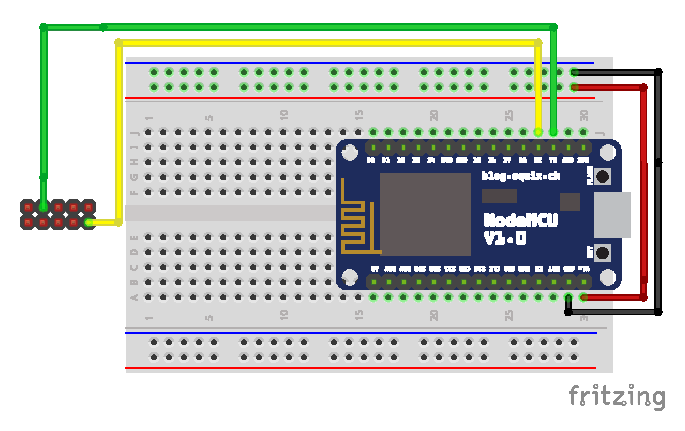
\includegraphics[width=\textwidth]{./05_c/figures/wsnWiring_Steckplatine.pdf}
		%\captionof{figure}{Verkabelung der Platinen}
		%\label{fig:wiring}
	\end{minipage}

	\item Um nun Daten in Form von Zeichenketten zu übertragen, muss zuerst die UART-Schnittstelle initialisiert werden. Dazu reicht es, den header \lstinline|uart_multicon.h| zu includen und die Funktion \lstinline|cpp_initUart3(115200)| aufzurufen. \lstinline|115200| ist die Baudrate mit der die Schnittstelle arbeiten muss.
	
	Zum übertragen von ganzen Zeichenketten, ist es hilfreich zunächst eine Funktion zu implementieren, welche ein einzelnes Zeichen entgegennimmt und überträgt (\zB \lstinline|void writeCharUart3(char c)|). In dieser Funktion muss gewartet werden, solange der Aufruf \lstinline|Mfs_Uart_GetStatus(\&UART3, UartTxEmpty)| nicht \lstinline|TRUE| ergibt. \lstinline|TRUE| ist in diesem Fall ein Makro der Treiberbibliothek, und muss daher genau so verwendet werden. Liefert der Aufruf \lstinline|FALSE| zurück, ist die Schnittstelle bereit um ein einzelnes Zeichen mit dem Aufruf von \lstinline|Mfs_Uart_SendData(\&UART3, c)| zu versenden.
	
	Implementiere nun noch eine Funktion die einen nullterminierten C-String entgegennimmt und durch wiederholte Aufrufe von \lstinline|writeCharUart(char c)| versendet.
	
	Teste deine Funktion, indem du ihr einen Text (\zB \lstinline|"mqtt_pub /Hello World!\r\n"|) übergibst. \lstinline|\r\n| markiert das Ende des Befehls. Auf der Serveranwendung sollte deine Nachricht nun ankommen.
	
	\item Erweitere nun dein Board um einen Sensor, und sende den gemessenen Sensorwert an die Zentrale Serveranwendung. Sende dazu den Befehl \lstinline|"mqtt_wsn <Sensorwert>\r\n"|.
	
	
\end{enumerate}



\cclicense

\end{document}
